%!TeX root=../tese.tex
%("dica" para o editor de texto: este arquivo é parte de um documento maior)
% para saber mais: https://tex.stackexchange.com/q/78101

%!TeX root=../tese.tex
%("dica" para o editor de texto: este arquivo é parte de um documento maior)
% para saber mais: https://tex.stackexchange.com/q/78101

\chapter{Conexidade em grafos dinâmicos}

\enlargethispage{.8\baselineskip}

Como citado no Capítulo~1, o problema da conexidade em grafos dinâmicos visa construir um algoritmo eficiente que dá suporte a inserções e remoções de arestas e consultas de conexidade entre dois vértices. O algoritmo de Holm, de Lichtenberg e Thorup~\cite{jacob_holm} para este problema de conexidade mantém $\left\lceil \lg n \right\rceil$ florestas dinâmicas do grafo $G$, e utiliza uma biblioteca que será descrita na próxima seção. 

\section{Conexidade em florestas dinâmicas}
\label{sec:dynamic-forest-connectivity}

Rodrigues \cite{arthur}, em sua dissertação do mestrado, estudou, entre outros assuntos, o problema da conexidade em florestas dinâmicas e implementou o algoritmo que foi proposto na Seção~2 do artigo de Holm, de Lichtenberg e Thorup~\cite{jacob_holm}. No Capítulo~2 da sua dissertação, Rodrigues descreve as rotinas principais de sua implementação, que se baseia em Euler tour trees, e realiza uma análise minuciosa da complexidade de tempo de cada rotina de sua implementação. Levando isso em conta, optamos por não apresentar uma descrição detalhada desse mesmo algoritmo, e apenas explicar brevemente o que as rotinas principais fazem, ressaltando algumas diferenças da nossa implementação em código em relação à de Rodrigues.  

O problema da conexidade em florestas dinâmicas pode ser considerado uma simplificação do problema de conexidade em grafos dinâmicos, quando o grafo em questão é uma floresta. A biblioteca que usaremos contém os seguintes métodos:

\begin{itemize}
    \item \texttt{\textbf{florestaDinâmica(n)}}: constrói e devolve uma floresta dinâmica $F$ com $n$ vértices e sem arestas;
    \item \texttt{\textbf{conectadosFD(F, u, v)}}: devolve verdadeiro se \textit{$u$} e \textit{$v$} estão na mesma componente da floresta $F$ e falso caso contrário;
    \item \texttt{\textbf{adicioneFD(F, u, v)}}: insere uma aresta \textit{uv} na floresta $F$;
    \item \texttt{\textbf{removaFD(u, v)}}: remove a aresta \textit{uv} da floresta $F$.
\end{itemize}


A estrutura de dados principal usada neste algoritmo de Holm, de Lichtenberg e Thorup~para dar suporte eficientes às rotinas acima é uma árvore binária de busca balanceada (ABBB). Dessa forma, a floresta dinâmica é constituída de várias ABBBs. Rodrigues utiliza \textit{treaps} em sua implementação, que são de natureza aleatória. Em nosso caso, utilizamos árvores \textit{splay}, que foram desenvolvidas por \textit{Sleator e Tarjan} \cite{sleator}. Árvores \textit{splay} são árvores binárias de busca (ABBs) que possuem uma rotina extra (além das usuais de busca, inserção e remoção) chamada \textit{splay}, que é acionada ao final de cada operação feita na árvore, de modo que é sempre aplicada ao nó mais profundo visitado. Isso faz com que o custo de uma sequência de $m$ operações (inserção, remoção ou busca) em uma árvore \textit{splay} com $n$ nós seja $\Oh(m\lg n)$, ou seja, o custo amortizado por operação é $\Oh(\lg n)$. Como também já existe bastante literatura sobre árvores \textit{splay}~\cite[Lecture 12]{kozen}, e seu funcionamento interno não afeta a descrição dos algoritmos que descreveremos, não entraremos em detalhes de sua implementação.

Nesse sentido, o resultado é uma implementação em que \texttt{florestaDinâmica(n)} tem custo $\Theta(n)$ e os demais métodos da biblioteca têm custo amortizado $\Oh(\lg n)$.

\section{Estrutura do grafo dinâmico}
\label{sec:dynamic-graph-structure}

Implementar o grafo dinâmico resume-se à construção da seguinte biblioteca de forma eficiente:

\begin{itemize}
    \item \texttt{\textbf{grafoDinâmico(n)}}: contrói e devolve um grafo dinâmico com $n$ vértices e sem arestas;
    \item \texttt{\textbf{conectadosGD(G, u, v)}}: devolve verdadeiro se os vértices $u$ e $v$ estão na mesma componente de $G$ e falso caso contrário;
    \item \texttt{\textbf{adicioneGD(G, u, v)}}: adiciona a aresta $uv$ no grafo $G$;
    \item \texttt{\textbf{removaGD(G, u, v)}}: remove a aresta $uv$ do grafo $G$.
\end{itemize} 

Para entender a base de como cada uma dessas rotinas funcionam, será necessário apresentar a estrutura interna da implementação do grafo para explicar como ele mantém essas estruturas e como elas deixam essas rotinas mais eficientes.

\subsection{Fatiamento do grafo em níveis}
\label{sec:level-slicing}

Na Seção~3.1 do artigo de Holm, de Lichtenberg e Thorup~\cite{jacob_holm}, é apresentada a técnica de fatiar o grafo $G$ em níveis. Cada aresta do grafo possui um nível entre $1$ e $\left\lceil \lg n \right\rceil$, onde $n$ é o número de vértices do grafo $G$. Toda vez que inserimos uma aresta em $G$, ela possuirá o nível $\left\lceil \lg n \right\rceil$, e ele nunca será aumentado. 

Seja $G$ um grafo com conjunto $V(G)$ de vértices e conjunto $E(G)$ de arestas. Se $X$ é um conjunto não-vazio de arestas, dizemos que o subgrafo de $G$ \textbf{induzido} por $X$ é o subgrafo gerador $H$ de $G$ tal que $E(H) = X$. Denotamos, $H$ como $G[X]$.

Sendo assim, seja $G_i = G[X]$ o grafo onde $X$ é o conjunto das arestas do grafo $G$ de nível menor ou igual a $i$. Para cada nível $i$, manteremos uma floresta maximal $F_i$ de $G_i$. Além disso, vamos manter também, para cada nível $i$, um grafo $R_i$ em forma de listas de adjacências, que guardam apenas arestas de nível $i$ que não estejam em $F_i$. 

Consequentemente, temos que $G_1 \subseteq G_2 \subseteq \cdots \subseteq G_{\left\lceil \lg n \right\rceil}$, para um grafo $G$ de $n$ vértices, e deduzimos que $G = G_{\left\lceil \lg n \right\rceil}$ e que $F_{\left\lceil \lg n \right\rceil}$ é uma floresta maximal de $G$. Dessa maneira, sempre que estivermos realizando alguma operação de consulta de conexidade em nosso grafo $G$, podemos realizá-la na floresta $F_{\left\lceil \lg n \right\rceil}$ de $G$.

Com isso, podemos estabelecer algumas invariantes, que são mantidas ao longo das modificações no grafo $G$:

\begin{enumerate}[label=(\Roman*)]
    \item \label{invariant1} $F_i$ é uma floresta maximal de $G_i$ para todo $1 \leq i \leq  \left\lceil \lg n \right\rceil$;
    
    \item \label{invariant2} $F_i \subseteq F_{i+1}$ para todo $1 \leq i \leq \left\lceil \lg n \right\rceil - 1$;
    
    \item \label{invariant3} Cada componente da floresta $F_i$ possui no máximo $2^i$ vértices.
\end{enumerate}

Na Seção~\ref{sec:dynamic-graph-routines}, descreveremos com mais detalhes como as rotinas da biblioteca funcionam e como cada uma preserva as invariantes acima, de modo a manter a corretude do algoritmo durante toda a sua execução.

Por fim, para simplificar um pouco a notação, escreveremos $L = \left\lceil \lg n \right\rceil$, isto é, $F_{\left\lceil \lg n \right\rceil}$ passa a ser escrita como $F_{L}$, da mesma forma que $G_L = G_{\left\lceil \lg n \right\rceil}$ e $R_L = R_{\left\lceil \lg n \right\rceil}$.

\subsection{Tipos de arestas do grafo}
\label{sec:dynamic-graph-edge-types}

% O objetivo de fatiar o grafo em  $\left\lceil \lg n \right\rceil$ níveis é para caso uma aresta da floresta de nível $i$ for removida, não será mais necessário procurar exaustivamente por substitutas nos níveis menores que $i$. Assim, passamos a buscar a substituta inicialmente nas arestas reservas em $R_i$. Caso não a encontremos, procuramos nas listas de adjacências $R_{i+1}, R_{i+2}, \ldots, R_{\left\lceil \lg n \right\rceil}$. Se não existir uma aresta substituta em $R_j$, $i \leq j \leq  \left\lceil \lg n \right\rceil$, então rebaixaremos as arestas que exploramos em $R_j$ de nível $j$ para um nível inferior $j-1$, caso $j > 0$. 

Quando realizamos uma chamada à função \texttt{adicioneGD($G$, $u$, $v$)}, é feita uma chamada à rotina \texttt{conectadosGD($G$, $u$, $v$)} para verificar a conexidade de $u$ com $v$ em $G$. Se estes vértices não estiverem na mesma componente de $G$, então a aresta $uv$ é inserida na floresta maximal $F_L$ que estamos mantendo, assim ligndo a árvore que contém $u$ com a que contém $v$ em $F_L$. Chamamos esse tipo de aresta de \textbf{aresta da floresta}.

Caso $u$ e $v$ já estejam conectados em $G$, então essa aresta $uv$ é chamada de \textbf{aresta reserva} e ela será armazenada no grafo $R_L$ representado por listas de adjacências, que contém a seguinte biblioteca:

\begin{itemize}
    \item \texttt{\textbf{listasDeAdjacências(n)}}: constrói e devolve um grafo com $n$ vértices e sem arestas, representado por listas de adjacências;
    \item \texttt{\textbf{adicioneLA(R, u, v)}}: adiciona $u$ na lista de adjacências de $v$ em $R$ e vice-versa;
    \item \texttt{\textbf{removaLA(R, u, v)}}: remove $u$ da lista de adjacências de $v$ em $R$ e vice-versa.
\end{itemize} 

A nossa implementação \cite{chung2025} de listas de adjacências possui um custo $\Oh(n)$ ao acionar o construtor \texttt{listasDeAdjacências}, e para 
as rotinas \texttt{adicioneLA} e \texttt{removaLA} é garantido tempo esperado $\Oh(1)$, visto que estamos utilizando um mapa hash da linguagem \textit{C++} para realizar adição de um vizinho $v$ na lista de $u$ e, remoção de $v$ da lista de adjacências de $u$.

\section{Rotinas da biblioteca do grafo dinâmico}
\label{sec:dynamic-graph-routines}

\subsection{Criação do grafo}
\label{sec:dynamic-graph-creation}

Para criar um grafo dinâmico $G$ com $n$ vértices e inicialmente sem arestas, chamamos a rotina \texttt{grafoDinâmico($n$)}, que por sua vez irá chamar \texttt{florestaDinâmica($n$)}, criando $\left\lceil \lg n \right\rceil$ florestas dinâmicas com $n$ vértices, e \texttt{listasDeAdjacências($n$)}, criando $\left\lceil \lg n \right\rceil$ grafos com $n$ vértices representados por listas de adjacências. 

Além disso, usamos um mapa hash para guardar e obter o nível de uma aresta $uv$ em tempo esperado $\Oh(1)$. Assim, este mapa usa como chave as pontas da aresta ($u$~e~$v$) e armazena o valor do nível da aresta $uv$. Assim, podemos definir um outro método \texttt{novoMapaHash($n$)} que devolve um mapa hash vazio para um grafo de $n$ vértices. Dessa forma, se chamarmos esse método e atribuirmos o objeto devolvido a uma variável chamada \textit{nível}, podemos realizar as seguintes operações com \textit{nível}:

\begin{itemize}
    \item \textit{nível[u, v]} $\leftarrow$ $i$: armazena $i$ como o nível da aresta $uv$.
    
    \item \textit{nível[u, v]} $\leftarrow$ \texttt{NIL}: remove a aresta $uv$ do mapa hash.
    
    \item $x$ $\leftarrow$ \textit{nível[u, v]}: atribui o valor do nível da aresta $uv$ à variável $x$. 
\end{itemize}

Dessa forma, podemos apresentar o construtor do grafo no Programa~\ref{prog:newGD}. 

\begin{programruledcaption}{\texttt{grafoDinâmico($n$)} \label{prog:newGD}}
    \noindent\textbf{Entrada}: Recebe o número $n$ de vértices do grafo. \\
    \textbf{Saída}: Devolve um grafo dinâmico $G$ com $n$ vértices e sem arestas.
    \vspace{-0.5\baselineskip}
    \begin{lstlisting}[
        language={[brazilian]pseudocode},
        style=pseudocode,
        style=wider,
        functions={},
        specialidentifiers={},
        escapeinside={(*@}{@*)},
    ]
    \textbf{para} $i$ := $1$ \textbf{até} $\left\lceil \lg n \right\rceil$ \textbf{faça}
        $G.F_i$ := \texttt{florestaDinâmica($n$)}
        $G.R_i$ := \texttt{listasDeAdjacências($n$)}
    G.nível := \texttt{novoMapaHash($n$)}
    devolva G
    \end{lstlisting}
    \vspace{-0.5\baselineskip}
\end{programruledcaption}

Como ambos \texttt{florestaDinâmica($n$)} e \texttt{listasDeAdjacências($n$)} consomem tempo $\Oh(n)$, então \texttt{grafoDinâmico($n$)} consome tempo $\Oh(n \lg n)$, pois estamos criando $\left\lceil \lg n \right\rceil$ florestas dinâmicas e listas de adjacências. Além disso, é fácil de ver que, ao final, as três invariantes valem.

\subsection{Consultas de conexidade no grafo dinâmico}
\label{sec:dynamic-graph-connectivity-queries}

Para testar a conexidade entre dois vértices $u$ e $v$ no grafo $G$, basta chamarmos \texttt{conectadosGD($G$, $u$, $v$)}, que por sua vez aciona \texttt{conectadosFD($F_L$, $u$, $v$)}, pois $F_L$ é uma floresta maximal de $G$ pelo invariante \ref{invariant1}. O Programa~\ref{prog:connectedGD} mostra essa rotina.

\begin{programruledcaption}{\texttt{conectadosGD($G$, $u$, $v$)} \label{prog:connectedGD}}
    \noindent\textbf{Entrada}: Recebe dois vértices $u$ e $v$ do grafo $G$. \\
    \textbf{Saída}: Devolve um booleano indicando se $u$ e $v$ estão conectados em $G$.
    \vspace{-0.5\baselineskip}
    \begin{lstlisting}[
        language={[brazilian]pseudocode},
        style=pseudocode,
        style=wider,
        functions={},
        specialidentifiers={},
        escapeinside={(*@}{@*)},
    ]
    devolva \texttt{conectadosFD($G.F_{\left\lceil \lg n \right\rceil}$, $u$, $v$)}
    \end{lstlisting}
    \vspace{-0.5\baselineskip}
\end{programruledcaption}

\raggedbottom


A rotina \texttt{conectadosFD($F_L$, $u$, $v$)} em nossa implementação consome tempo amortizado $\Oh(\lg n)$, e, portanto, \texttt{conectadosGD($F_L$, $u$, $v$)} também terá o mesmo consumo de tempo amortizado.
Além disso, a rotina de consulta não altera o nosso grafo, incluindo florestas e listas de adjacências, já que não há nenhuma modificação neles. Isso implica que as invariantes são mantidas. 









\subsection{Inserções de arestas no grafo dinâmico}

Como explicado na Seção~\ref{sec:dynamic-graph-edge-types}, inserimos uma aresta $uv$ no grafo $G$ chamando a rotina \texttt{adicioneGD($G$, $u$, $v$)} e, em seguida, testamos a conexidade de $u$ e $v$ chamando a rotina \texttt{conectadosGD($G$, $u$, $v$)}, e, dependendo do resultado, $uv$ pode ser inserida como aresta reserva ou como aresta da floresta. Assumindo que a aresta $uv$ não exista em $G$ no momento de sua inserção, temos dois cenários:

\begin{itemize}
    \item 
    Se os vértices $u$ e $v$ já estão conectados em $G$, então chamaremos a função \texttt{adicioneLA($R_L$, $u$, $v$)}, que irá armazenar $uv$ como aresta reserva de nível $L$ de $G$ em $R_L$. A Figura~\ref{fig:graph_reserve_edge_uv_addition} ilustra esse cenário.

\end{itemize}

\begin{figure}[H]
    \centering
    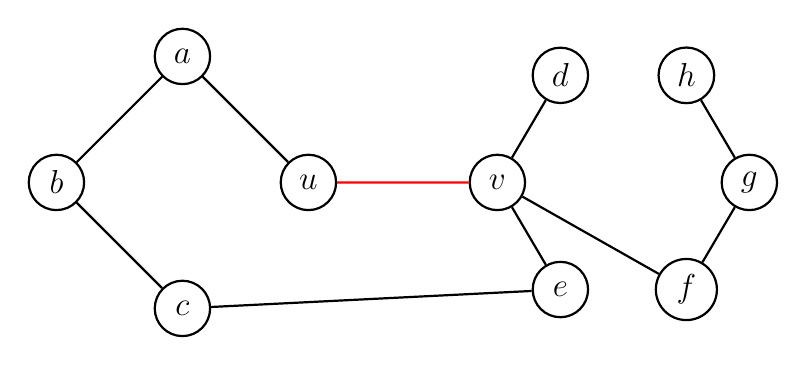
\begin{tikzpicture}
        [scale=0.8, node/.style={circle,draw,minimum size=2em, thick, font=\large},
        edge/.style={thick, black},
        reserve/.style={red, thick},
        removed/.style={black, thick, dashed}]

        \node[node] (u) at (-1,2) {$u$};
        \node[node] (a) at (-3,4) {$a$};
        \node[node] (b) at (-5,2) {$b$};
        \node[node] (c) at (-3,0) {$c$};
        \node[node] (v) at (2,2) {$v$};
        \node[node] (d) at (3,3.7) {$d$};
        \node[node] (e) at (3,0.3) {$e$};
        \node[node] (f) at (5,0.3) {$f$};
        \node[node] (g) at (6, 2) {$g$};
        \node[node] (h) at (5, 3.7) {$h$};
        
        

        % tree edges (normal black edges)
        \draw[edge] (a) -- (u) node[midway, below] {};
        \draw[edge] (a) -- (b) node[midway, below] {};
        \draw[edge] (b) -- (c) node[midway, below] {};
        \draw[edge] (v) -- (d) node[midway, below] {};
        \draw[edge] (v) -- (f) node[midway, below] {};
        \draw[edge] (v) -- (e) node[midway, below] {};
        \draw[edge] (c) -- (e) node[midway, below] {};
        \draw[edge] (f) -- (g) node[midway, below] {};
        \draw[edge] (g) -- (h) node[midway, below] {};

        % reserve edges (normal red edges)
        \draw[reserve] (u) -- (v) node[midway, below] {};


    \end{tikzpicture}
    \caption{As arestas pretas são da floresta maximal $F_L$ do grafo. Como queremos inserir a aresta $uv$ e os vértices $u$ e $v$ já estão conectados pelo caminho $u \rightarrow a \rightarrow b \rightarrow c \rightarrow e \rightarrow v$, então armazenamos $uv$ como aresta reserva (em vermelho).}
    \label{fig:graph_reserve_edge_uv_addition}
\end{figure}

\begin{itemize}
    \item  Se $u$ e $v$ não estão conectados em $G$, então inserimos $uv$ como aresta da floresta $F_L$ de nível $L$, chamando a função \texttt{adicioneFD($F_L$, $u$, $v$)}. A Figura~\ref{fig:graph_tree_edge_uv_addition} ilustra esse cenário.
\end{itemize}

\begin{figure}[H]
    \centering
    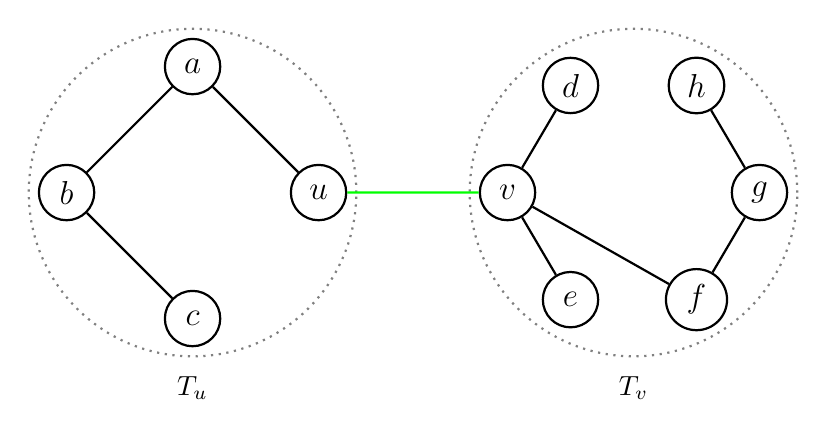
\begin{tikzpicture}
        [scale=0.8, node/.style={circle,draw,minimum size=2em, thick, font=\large},
        edge/.style={thick, black},
        added/.style={thick, green},
        reserve/.style={red, thick},
        removed/.style={black, thick, dashed}]

        \node[node] (u) at (-1,2) {$u$};
        \node[node] (a) at (-3,4) {$a$};
        \node[node] (b) at (-5,2) {$b$};
        \node[node] (c) at (-3,0) {$c$};
        \node[node] (v) at (2,2) {$v$};
        \node[node] (d) at (3,3.7) {$d$};
        \node[node] (e) at (3,0.3) {$e$};
        \node[node] (f) at (5,0.3) {$f$};
        \node[node] (g) at (6, 2) {$g$};
        \node[node] (h) at (5, 3.7) {$h$};
        
        
         % Dotted circles for T_u and T_v
        \draw[dotted, thick, gray] (-3,2) circle (2.6cm);
        \draw[dotted, thick, gray] (4,2) circle (2.6cm);  
        
        % Labels for the circles
        \node at (-3,-1.1) {$T_u$};
        \node at (4,-1.1) {$T_v$};

        % tree edges (normal black edges)
        \draw[edge] (a) -- (u) node[midway, below] {};
        \draw[edge] (a) -- (b) node[midway, below] {};
        \draw[edge] (b) -- (c) node[midway, below] {};
        \draw[edge] (v) -- (d) node[midway, below] {};
        \draw[edge] (v) -- (f) node[midway, below] {};
        \draw[edge] (v) -- (e) node[midway, below] {};
        \draw[edge] (f) -- (g) node[midway, below] {};
        \draw[edge] (g) -- (h) node[midway, below] {};
        \draw[added] (u) -- (v) node[midway, below] {};

        % reserve edges (normal red edges)


    \end{tikzpicture}
    \caption{As arestas pretas são da floresta maximal $F_L$ do grafo. Como os vértices $u$ e $v$ não estão conectados em $F_L$, então inserimos $uv$ como aresta da floresta (em verde), nesse caso conectando as componentes $T_u$ e $T_v$ de $F_L$.}
    \label{fig:graph_tree_edge_uv_addition}
\end{figure}

O Programa~\ref{prog:addGD} ilustra uma primeira versão da rotina \texttt{adicioneGD}. Posteriormente, faremos alguns ajustes nessa rotina por causa da rotina de remoção de arestas explicada na Seção~\ref{sec:dynamic-graph-edge-removal}.

\begin{programruledcaption}{\texttt{adicioneGD($G$, $u$, $v$)} \label{prog:addGD}}
    \noindent\textbf{Entrada}: Recebe dois vértices $u$ e $v$ do grafo $G$. \\
    \textbf{Efeito}: Adiciona a aresta $uv$ no grafo $G$.
    \vspace{-0.5\baselineskip}
    \begin{lstlisting}[
        language={[brazilian]pseudocode},
        style=pseudocode,
        style=wider,
        functions={},
        specialidentifiers={},
        escapeinside={(*@}{@*)},
    ]
    G.nível[u, v] := $\left\lceil \lg n \right\rceil$
    \textbf{se} \texttt{conectadosFD($G.F_{\left\lceil \lg n \right\rceil}$, $u$, $v$)} \textbf{então}
        \texttt{adicioneLA($G.R_{\left\lceil \lg n \right\rceil}$, $u$, $v$)}
    \textbf{senão}
        \texttt{adicioneFD($G.F_{\left\lceil \lg n \right\rceil}$, $u$, $v$)}
    \end{lstlisting}
    \vspace{-0.5\baselineskip}
\end{programruledcaption}

\raggedbottom

% Ao inserirmos uma aresta reserva $uv$ em $G$, precisamos atualizar o atributo \textit{incideArestaReservaDeNível} de $u$ e de $v$ para verdadeiro, se necessário. A Seção~\ref{sec:graph-nodes} explica com mais detalhes o método auxiliar (\texttt{incrementeArestasReservasDeNível}) usado. 

Em nossa implementação, \texttt{conectadosGD} consome tempo amortizado $\Oh(\lg n)$. A rotina \texttt{adicioneLA}, quando acionada, consome tempo esperado constante $\Oh(1)$ em nossa implementação por conta do mapa hash. Já inserir uma aresta da floresta chamando \texttt{adicioneFD} consome tempo $\Oh(\lg n)$ (amortizado, em nossa implementação). Portanto, o custo de tempo ao acionar a rotina \texttt{adicioneGD} será amortizado $\Oh(\lg n)$.

A invariante \ref{invariant1} se mantém para o nível $i = \left\lceil \lg n \right\rceil$. Como sempre adicionamos arestas com nível $\left\lceil \lg n \right\rceil$ em $F_{\left\lceil \lg n \right\rceil}$ (se não forem reservas), então as outras florestas de níveis inferiores não são afetadas, mantendo-se, assim, os invariantes \ref{invariant2} e \ref{invariant3} também.























































\subsection{Remoção de arestas no grafo dinâmico}
\label{sec:dynamic-graph-edge-removal}

A remoção de arestas se divide em dois casos: remoção de uma aresta reserva ou remoção de uma aresta da floresta.

Quando queremos remover uma aresta $uv$ e ela é reserva, podemos simplesmente acionar a rotina \texttt{removaLA($R_i$, $u$, $v$)} onde $i$, obtido do mapa hash, é o nível da aresta a ser removida e $R_i$ é a lista de adjacências na qual $uv$ está armazenada. Por conta disso, nenhuma das florestas maximais $F_j$ do grafo será afetada, e as três invariantes serão mantidas. A Figura~\ref{fig:graph_reserve_edge_removal} mostra esse cenário apresentado.

\begin{figure}[H]
    \centering
    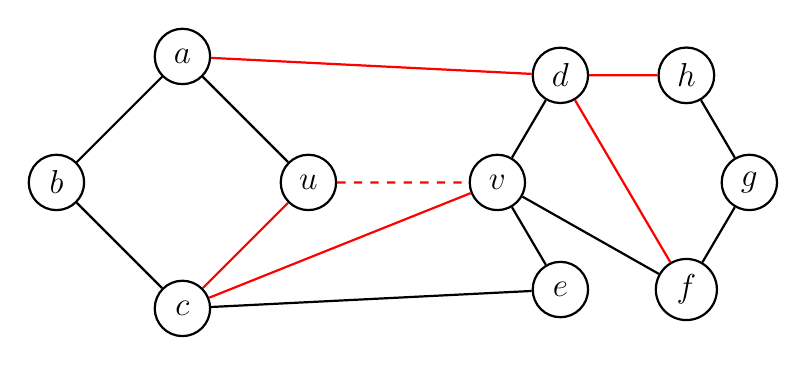
\begin{tikzpicture}
        [scale=0.8, node/.style={circle,draw,minimum size=2em, thick, font=\large},
        edge/.style={thick, black},
        reserve/.style={red, thick},
        removed/.style={black, thick, dashed},
        removed_reserve/.style={red, thick, dashed}]

        \node[node] (u) at (-1,2) {$u$};
        \node[node] (a) at (-3,4) {$a$};
        \node[node] (b) at (-5,2) {$b$};
        \node[node] (c) at (-3,0) {$c$};
        \node[node] (v) at (2,2) {$v$};
        \node[node] (d) at (3,3.7) {$d$};
        \node[node] (e) at (3,0.3) {$e$};
        \node[node] (f) at (5,0.3) {$f$};
        \node[node] (g) at (6, 2) {$g$};
        \node[node] (h) at (5, 3.7) {$h$};
        

        % tree edges (normal black edges)
        \draw[edge] (a) -- (u) node[midway, below] {};
        \draw[edge] (a) -- (b) node[midway, below] {};
        \draw[edge] (b) -- (c) node[midway, below] {};
        \draw[edge] (v) -- (d) node[midway, below] {};
        \draw[edge] (v) -- (f) node[midway, below] {};
        \draw[edge] (v) -- (e) node[midway, below] {};
        \draw[edge] (c) -- (e) node[midway, below] {};
        \draw[edge] (f) -- (g) node[midway, below] {};
        \draw[edge] (g) -- (h) node[midway, below] {};

        % reserve edges (normal red edges)
        \draw[reserve] (a) -- (d) node[midway, below] {};
        \draw[reserve] (c) -- (v) node[midway, below] {};
        \draw[removed_reserve] (u) -- (v) node[midway, below] {};
        \draw[reserve] (c) -- (u) node[midway, below] {};
        \draw[reserve] (d) -- (f) node[midway, below] {};
        \draw[reserve] (d) -- (h) node[midway, below] {};

    \end{tikzpicture}
    \caption{As arestas pretas são da floresta maximal $F_L$ do grafo, enquanto as vermelhas são arestas reservas. A aresta vermelha $uv$ tracejada é reserva e está prestes a ser removida.}
    \label{fig:graph_reserve_edge_removal}
\end{figure}

O caso da remoção de uma aresta $uv$ da floresta é mais complexo. Se a aresta $uv$ tem nível $i$, remover $uv$ sempre quebra uma componente de $F_i$ em duas árvores $T_u$ e $T_v$, de modo que a primeira contém o vértice $u$ e a segunda contém o vértice $v$. Neste caso, precisamos verificar se existe alguma aresta reserva que ligue $T_u$ a $T_v$, para que possamos garantir que a floresta $F_i$ continue maximal em $G_i$. Chamamos uma tal aresta de \textbf{aresta substituta}.

\begin{figure}[H]
    \centering
    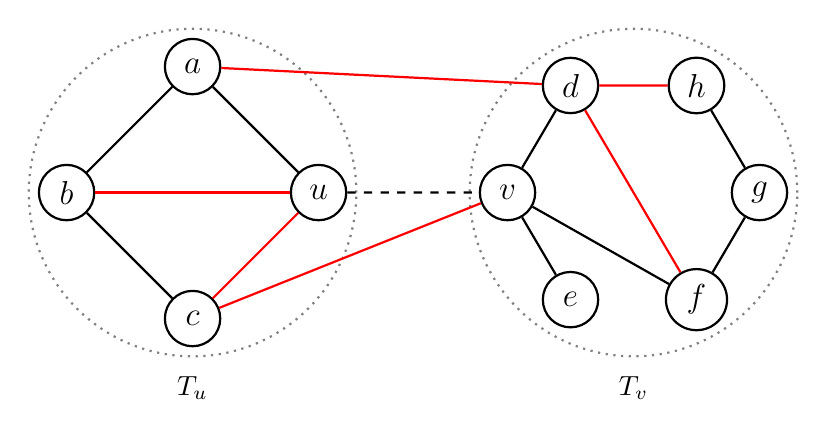
\begin{tikzpicture}
        [scale=0.8, node/.style={circle,draw,minimum size=2em, thick, font=\large},
        edge/.style={thick, black},
        reserve/.style={red, thick},
        removed/.style={black, thick, dashed}]

        \node[node] (u) at (-1,2) {$u$};
        \node[node] (a) at (-3,4) {$a$};
        \node[node] (b) at (-5,2) {$b$};
        \node[node] (c) at (-3,0) {$c$};
        \node[node] (v) at (2,2) {$v$};
        \node[node] (d) at (3,3.7) {$d$};
        \node[node] (e) at (3,0.3) {$e$};
        \node[node] (f) at (5,0.3) {$f$};
        \node[node] (g) at (6, 2) {$g$};
        \node[node] (h) at (5, 3.7) {$h$};
        
        
         % Dotted circles for T_u and T_v
        \draw[dotted, thick, gray] (-3,2) circle (2.6cm);
        \draw[dotted, thick, gray] (4,2) circle (2.6cm);  
        
        % Labels for the circles
        \node at (-3,-1.1) {$T_u$};
        \node at (4,-1.1) {$T_v$};

        % tree edges (normal black edges)
        \draw[edge] (a) -- (u) node[midway, below] {};
        \draw[edge] (a) -- (b) node[midway, below] {};
        \draw[edge] (b) -- (c) node[midway, below] {};
        \draw[edge] (v) -- (d) node[midway, below] {};
        \draw[edge] (v) -- (f) node[midway, below] {};
        \draw[edge] (v) -- (e) node[midway, below] {};
        \draw[removed] (u) -- (v) node[midway, above] {};
        \draw[edge] (f) -- (g) node[midway, below] {};
        \draw[edge] (g) -- (h) node[midway, below] {};
        \draw[reserve] (a) -- (d) node[midway, below] {};
        \draw[reserve] (c) -- (v) node[midway, below] {};

        % reserve edges (normal red edges)
        \draw[reserve] (b) -- (u) node[midway, below] {};
        \draw[reserve] (c) -- (u) node[midway, below] {};
        \draw[reserve] (d) -- (f) node[midway, below] {};
        \draw[reserve] (d) -- (h) node[midway, below] {};

    \end{tikzpicture}
    \caption{As arestas pretas são da floresta maximal $F_i$ do grafo $G_i$, enquanto as vermelhas são reservas de nível $i$. A aresta $uv$ tracejada de nível $i$ está prestes a ser removida, assim ela pode ser substituída por $ad$ ou $cv$, pois qualquer uma destas liga $T_u$ a $T_v$.}
    \label{fig:graph_with_Tu_and_Tv_with_reserve_edge}
\end{figure}

Para buscar uma aresta reserva de maneira o mais eficiente possível, o algoritmo percorre cada vértice $x$ de $T_u$ e verifica se existe algum vértice $y$ na lista de adjacência de $x$ de $R_i$ que esteja em $T_v$. Se $y \in V(T_v)$, então a aresta $xy$ é uma aresta substituta $R_i$ de nível $i$, bastando apenas acionar \texttt{adicioneFD($F_i$, $x$, $y$)} para reconectar $T_u$ e $T_v$, que virariam uma única componente da floresta $F_i$, e acionar \texttt{removaLA($R_i$, $x$, $y$)} já que $xy$ se tornará uma aresta da floresta.

É por este motivo que introduzimos o fatiamento em níveis na Seção~\ref{sec:level-slicing}. A intuição por trás deste fatiamento é que, quando uma aresta de nível $i$ da floresta é removida, não é necessário buscar por substitutas nos níveis menores que $i$. Isso quer dizer que começamos a busca no nível em questão, ou seja, em $R_i$, e caso não haja nenhuma substituta em $R_i$, passamos a procurar em $R_{i+1}, R_{i + 2}, \ldots, R_L$. Quando não encontramos uma substituta em um certo $R_i$, aproveitamos para rebaixar o nível de todas as arestas percorridas em $R_i$ para $i - 1$, de modo que não precisaremos mais percorrer essas arestas quando removermos uma outra aresta de nível $i$, visto que elas já estariam em $R_{i-1}$.


Na verdade, antes de fazer esse rebaixamento, rebaixamos o nível de toda aresta de nível $i$ de $T_u$ para $i-1$, de modo que $T_u \subseteq F_{i-1}$.
Rebaixar o nível dessas arestas significa inseri-las em $F_{i-1}$, pois elas passam a ser de nível $i-1$. Esse rebaixamento e as inserções em $F_{i-1}$ se tornam necessários para preservar a invariante~\ref{invariant1}. Ao mesmo tempo, para manter também a invariante~\ref{invariant3}, esse processo deverá ser feito na menor das árvores $T_u$ e $T_v$. Seja $T = T_u \cup T_v$. Denotando o número de vértices de uma árvore $T$ por $|T|$, o algoritmo garantirá que $|T_u| \leq |T_v|$. Pela invariante~\ref{invariant3}, temos que $|T| \leq 2^i$, e como $|T_u| + |T_v| = |T|$, então $|T_u| \leq 2^{i-1}$. Por isso, ao rebaixarmos todas as arestas de nível $i$ de $T_u$ para o nível $i-1$, preservamos a invariante~\ref{invariant3}. 

Ao remover uma aresta de nível $i$ da floresta, na verdade temos que removê-la não só de $F_i$, mas também de $F_{i + 1}, \ldots, F_{L}$ pela invariante~\ref{invariant2}. Similarmente, quando encontramos uma aresta substituta de nível $i$, temos que acrescentá-la não só a $F_i$, mas também a $F_{i+1}, \ldots, F_{L}$ para manter as invariantes~\ref{invariant1} e \ref{invariant2}. A invariante~\ref{invariant3} neste caso é mantida trivialmente.

Agora, veremos em detalhes o motivo de não precisarmos procurar uma substituta em níveis menores que $i$ quando removemos uma aresta $uv$ de nível $i$. Veja que, como a aresta $uv$ tem nível $i$, ela não pertence a $F_{i-1}$. Logo, pela invariante~\ref{invariant2}, $u$ e $v$ estão em componentes distintas de $F_{i-1}$. Como $F_{i-1}$ é maximal em $G_{i-1}$, não existe aresta reserva de nível $\leq i - 1$ que conecte as componentes $T_u$ e $T_v$. Portanto, só procuramos uma substituta em níveis $\geq i$. A Figura~\ref{fig:why-not-search-in-less-or-equal-than-i} torna a explicação mais intuitiva.

\begin{figure}[H]
    \centering
    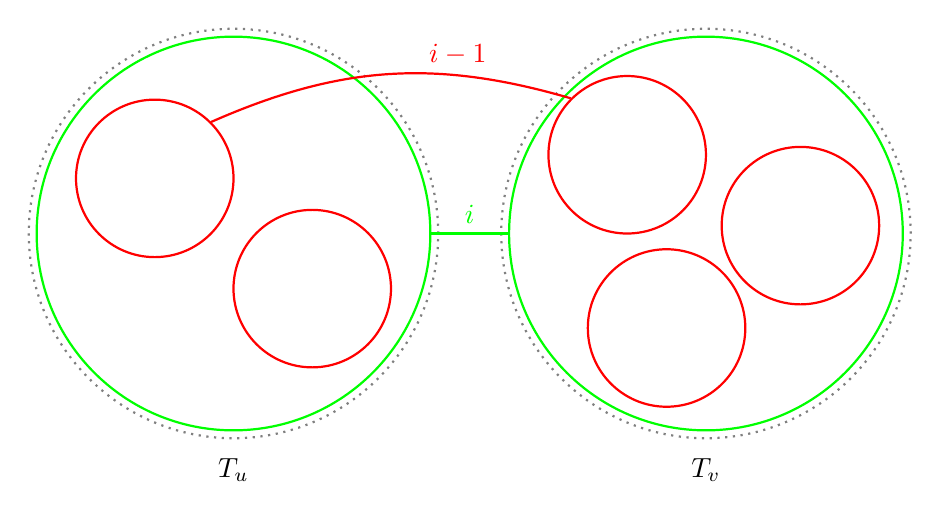
\begin{tikzpicture}[>=stealth, thick]

    % Big green circles g1 and g2
    \node[draw, thick, green, circle, minimum size=5cm] (g1) at (-3,0) {};
    \node[draw, thick, green, circle, minimum size=5cm] (g2) at (3,0) {};

    \draw[dotted, thick, gray] (-3,0) circle (2.6cm);
    \draw[dotted, thick, gray] (3,0) circle (2.6cm);  
    
    % Labels for the circles
    \node at (-3,-3) {$T_u$};
    \node at (3, -3) {$T_v$};

    % Straight green edge between g1 and g2
    \draw[thick, green] (g1) -- node[above] {$i$} (g2);

    % Small red circles inside g1
    \node[draw, thick, red, circle, minimum size=2cm] (r11) at (-4,0.7) {};
    \node[draw, thick, red, circle, minimum size=2cm] (r12) at (-2,-0.7) {};

    % Small red circles inside g2
    \node[draw, thick, red, circle, minimum size=2cm] (r21) at (2,1) {};
    \node[draw, thick, red, circle, minimum size=2cm] (r22) at (4.2,0.1) {};
    \node[draw, thick, red, circle, minimum size=2cm] (r23) at (2.5,-1.2) {};

    % Curved red edge connecting one red circle in g1 with one in g2
    \draw[thick, red] (r11.north east) to[bend left=20] node[pos=0.7, above] {$i-1$} (r21.north west);

    \end{tikzpicture}
    \caption{Os círculos verdes representam as componentes da floresta $F_i$ do grafo $G_i$, enquanto os círculos vermelhos representam as componentes da floresta $F_{i-1}$ do grafo $G_{i-1}$. Note que a aresta reserva de nível $i-1$ mostrada não deveria existir, porque senão ela violaria a invariante~\ref{invariant1}. Portanto, tais arestas de nível $i-1$ ligando componentes de $F_i$ (como a aresta vermelha) não existem e só é necessário procurar arestas substitutas a partir de nível $i$ (como a aresta verde) para conectar as duas componentes $T_u$ e $T_v$.}
    \label{fig:why-not-search-in-less-or-equal-than-i}
\end{figure}

\raggedbottom

A seguir, demonstraremos a remoção de uma aresta $uv$ da floresta em uma série de imagens. Na Figura~\ref{fig:example-replacement1}, temos um grafo $G$ de $n = 10$ vértices. Para facilitar, assumiremos que, até o momento, só houve inserções de arestas. 

\begin{figure}[H]
    \centering

    \noindent
    \begin{minipage}[c]{2cm}
        \raggedright
        Nível $4$
    \end{minipage}%
    \begin{minipage}[c]{0.8\textwidth}
        \centering
        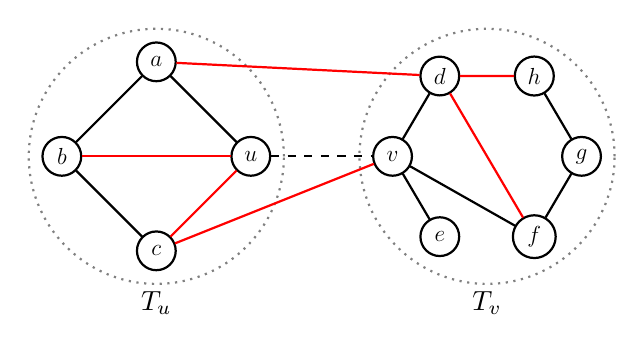
\begin{tikzpicture}
        [scale=0.6, node/.style={scale=0.7, circle,draw,minimum size=2em, thick, font=\large},
        edge/.style={thick, black},
        reserve/.style={red, thick},
        removed/.style={black, thick, dashed}]

        \node[node] (u) at (-1,2) {$u$};
        \node[node] (a) at (-3,4) {$a$};
        \node[node] (b) at (-5,2) {$b$};
        \node[node] (c) at (-3,0) {$c$};
        \node[node] (v) at (2,2) {$v$};
        \node[node] (d) at (3,3.7) {$d$};
        \node[node] (e) at (3,0.3) {$e$};
        \node[node] (f) at (5,0.3) {$f$};
        \node[node] (g) at (6, 2) {$g$};
        \node[node] (h) at (5, 3.7) {$h$};
        
         % Dotted circles for T_u and T_v
        \draw[dotted, thick, gray] (-3,2) circle (2.7cm);
        \draw[dotted, thick, gray] (4,2) circle (2.7cm);  
        
        % Labels for the circles
        \node at (-3,-1.1) {$T_u$};
        \node at (4,-1.1) {$T_v$};

        % tree edges (normal black edges)
        \draw[edge] (a) -- (u) node[midway, below] {};
        \draw[edge] (a) -- (b) node[midway, below] {};
        \draw[edge] (b) -- (c) node[midway, below] {};
        \draw[edge] (v) -- (d) node[midway, below] {};
        \draw[edge] (v) -- (f) node[midway, below] {};
        \draw[edge] (v) -- (e) node[midway, below] {};
        \draw[edge] (f) -- (g) node[midway, below] {};
        \draw[edge] (g) -- (h) node[midway, below] {};
        % reserve edges (normal red edges)
        
        \draw[removed] (u) -- (v) node[midway, below] {};
        \draw[reserve] (a) -- (d) node[midway, below] {};
        \draw[reserve] (c) -- (v) node[midway, below] {};
        \draw[reserve] (b) -- (u) node[midway, below] {};
        \draw[reserve] (c) -- (u) node[midway, below] {};
        \draw[reserve] (d) -- (f) node[midway, below] {};
        \draw[reserve] (d) -- (h) node[midway, below] {};

        \end{tikzpicture}
    \end{minipage}
    \vspace{1cm}
        \noindent
    \begin{minipage}[c]{2cm}
        \raggedright
        Nível $3$
    \end{minipage}%
    \begin{minipage}[c]{0.8\textwidth}
        \centering
        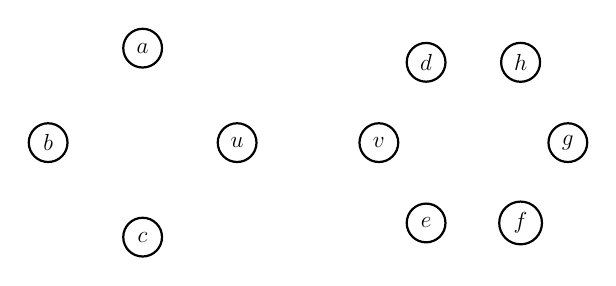
\begin{tikzpicture}
            [scale=0.6, node/.style={scale=0.7, circle,draw,minimum size=2em, thick, font=\large},
            edge/.style={thick, black},
            reserve/.style={red, thick},
            removed/.style={black, thick, dashed}]

            \node[node] (u) at (-1,2) {$u$};
            \node[node] (a) at (-3,4) {$a$};
            \node[node] (b) at (-5,2) {$b$};
            \node[node] (c) at (-3,0) {$c$};
            \node[node] (v) at (2,2) {$v$};
            \node[node] (d) at (3,3.7) {$d$};
            \node[node] (e) at (3,0.3) {$e$};
            \node[node] (f) at (5,0.3) {$f$};
            \node[node] (g) at (6, 2) {$g$};
            \node[node] (h) at (5, 3.7) {$h$};
            
            %\draw[edge] (a) -- (u) node[midway, below] {};
            %\draw[edge] (a) -- (b) node[midway, below] {};
            %\draw[edge] (b) -- (c) node[midway, below] {};

        \end{tikzpicture}
    \end{minipage}
    \caption{Um grafo $G$ de 10 vértices, onde as arestas pretas são da floresta $F_4$, enquanto as vermelhas são reservas. A aresta $uv$ está prestes a ser removida. A floresta $F_{4}$ de $G$ de cima contém todas as arestas pretas recém-inseridas e as arestas vermelhas estão em $R_4$. A floresta de baixo é a $F_{3}$, com os vértices isolados, e $R_3$ também não tem nenhuma aresta.}
    \vspace{-1cm}
    \label{fig:example-replacement1}
\end{figure}

\raggedbottom

Temos também que $n = 10$ e $\left\lceil \lg 10 \right\rceil = 4$, logo o nível máximo $L$ da floresta é $4$ e,  consequentemente, $G = G_4$. Como todas as inserções só acontecem no nível $L$, no momento, em $F_4$, só temos arestas da floresta de nível $4$, enquanto $F_3$ contém apenas vértices isolados. Neste cenário, note que a remoção da aresta $uv$ da floresta, representada por uma linha tracejada na figura, acaba quebrando a única componente da floresta $F_4$ em duas, $T_u$ e $T_v$. Como $F_4$ é a floresta maximal de nível máximo de $G$, então removemos somente a $uv$ de $F_4$. 

O próximo passo é rebaixar o nível de todas as arestas de nível~$4$ em $T_u$ para o nível $3$. Dessa forma, as arestas de $T_u$ passam a estar em $F_3$, como se pode ver na Figura~\ref{fig:example-replacement2}, pois agora elas passam a ser de nível $3$.  

Perceba que, devido à invariante~\ref{invariant2}, podemos ter arestas de diferentes níveis em uma mesma floresta. Assim, percorrer todas as arestas de $T_u$ e selecionar apenas as de nível $i$ para rebaixar pode se tornar demorado quando o grafo possui uma grande quantidade de arestas. A forma como o algoritmo procura as arestas de nível $i$ de $T_u$ será descrita de maneira mais detalhada na Seção~\ref{sec:node-edge}. No momento, só precisamos entender como este rebaixamento funciona.

\begin{figure}[H]
    \centering

    \noindent
    \begin{minipage}[c]{2cm}
        \raggedright
        Nível $4$
    \end{minipage}%
    \begin{minipage}[c]{0.8\textwidth}
        \centering
        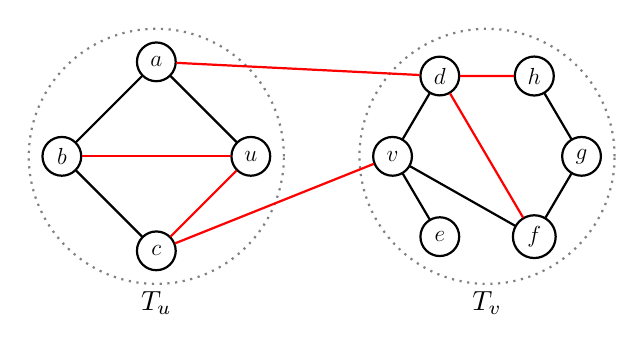
\begin{tikzpicture}
        [scale=0.6, node/.style={scale=0.7, circle,draw,minimum size=2em, thick, font=\large},
        edge/.style={thick, black},
        reserve/.style={red, thick},
        removed/.style={black, thick, dashed}]

        \node[node] (u) at (-1,2) {$u$};
        \node[node] (a) at (-3,4) {$a$};
        \node[node] (b) at (-5,2) {$b$};
        \node[node] (c) at (-3,0) {$c$};
        \node[node] (v) at (2,2) {$v$};
        \node[node] (d) at (3,3.7) {$d$};
        \node[node] (e) at (3,0.3) {$e$};
        \node[node] (f) at (5,0.3) {$f$};
        \node[node] (g) at (6, 2) {$g$};
        \node[node] (h) at (5, 3.7) {$h$};
        
         % Dotted circles for T_u and T_v
        \draw[dotted, thick, gray] (-3,2) circle (2.7cm);
        \draw[dotted, thick, gray] (4,2) circle (2.7cm);  
        
        % Labels for the circles
        \node at (-3,-1.1) {$T_u$};
        \node at (4,-1.1) {$T_v$};

        % tree edges (normal black edges)
        \draw[edge] (a) -- (u) node[midway, below] {};
        \draw[edge] (a) -- (b) node[midway, below] {};
        \draw[edge] (b) -- (c) node[midway, below] {};
        \draw[edge] (v) -- (d) node[midway, below] {};
        \draw[edge] (v) -- (f) node[midway, below] {};
        \draw[edge] (v) -- (e) node[midway, below] {};
        \draw[edge] (f) -- (g) node[midway, below] {};
        \draw[edge] (g) -- (h) node[midway, below] {};
        % reserve edges (normal red edges)
        
        \draw[reserve] (a) -- (d) node[midway, below] {};
        \draw[reserve] (c) -- (v) node[midway, below] {};
        \draw[reserve] (b) -- (u) node[midway, below] {};
        \draw[reserve] (c) -- (u) node[midway, below] {};
        \draw[reserve] (d) -- (f) node[midway, below] {};
        \draw[reserve] (d) -- (h) node[midway, below] {};

        \end{tikzpicture}
    \end{minipage}
    \vspace{1cm}
        \noindent
    \begin{minipage}[c]{2cm}
        \raggedright
        Nível $3$
    \end{minipage}%
    \begin{minipage}[c]{0.8\textwidth}
        \centering
        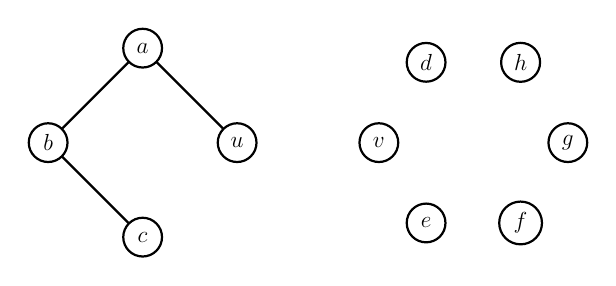
\begin{tikzpicture}
            [scale=0.6, node/.style={scale=0.7, circle,draw,minimum size=2em, thick, font=\large},
            edge/.style={thick, black},
            reserve/.style={red, thick},
            removed/.style={black, thick, dashed}]

            \node[node] (u) at (-1,2) {$u$};
            \node[node] (a) at (-3,4) {$a$};
            \node[node] (b) at (-5,2) {$b$};
            \node[node] (c) at (-3,0) {$c$};
            \node[node] (v) at (2,2) {$v$};
            \node[node] (d) at (3,3.7) {$d$};
            \node[node] (e) at (3,0.3) {$e$};
            \node[node] (f) at (5,0.3) {$f$};
            \node[node] (g) at (6, 2) {$g$};
            \node[node] (h) at (5, 3.7) {$h$};
            
            
            \draw[edge] (a) -- (u) node[midway, below] {};
            \draw[edge] (a) -- (b) node[midway, below] {};
            \draw[edge] (b) -- (c) node[midway, below] {};

        \end{tikzpicture}
    \end{minipage}
    \caption{Representação da remoção da aresta $uv$ em $G$. As arestas de nível $4$ de $T_u$ foram rebaixadas para o nível $3$, o que pode ser visto na floresta $F_{3}$.}
    \vspace{-1cm}
    \label{fig:example-replacement2}    
\end{figure}

\raggedbottom

Como $T_u$ e $T_v$ em $F_4$ ficaram separadas após a remoção de $uv$, precisamos descobrir, se existir, uma aresta reserva que possa reconectá-las. Note que percorrer todas as arestas reservas para achar uma substituta que ligue $T_u$ a $T_v$ pode ser ineficiente quando temos muitas arestas reservas. Por isso, explicaremos como implementar essa busca por uma substituta de forma eficiente na Seção~\ref{sec:node-vertex}. 

Na Figura~\ref{fig:example-replacement3}, percorremos as arestas reservas em $R_4$ que tenham uma das pontas em $T_u$. Para cada aresta percorrida, verificamos se a outra ponta dela incide em algum vértice de $T_v$. Caso não incida, a aresta tem duas pontas em $T_u$, pois $T_u$ é maximal em $F_4$, e logo a aresta não é uma substituta.  Então a rebaixamos para o nível $3$, ou seja, movemos de $R_4$ para $R_3$ as arestas  percorridas que não são substitutas e inserimos em $R_3$.

\begin{figure}[H]
    \centering

    \noindent
    \begin{minipage}[c]{2cm}
        \raggedright
        Nível $4$
    \end{minipage}%
    \begin{minipage}[c]{0.8\textwidth}
        \centering
        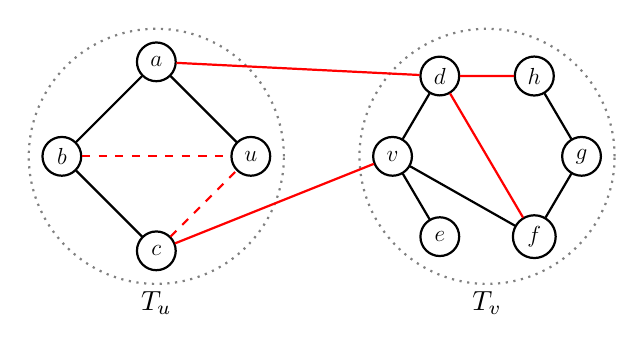
\begin{tikzpicture}
        [scale=0.6, node/.style={scale=0.7, circle,draw,minimum size=2em, thick, font=\large},
        edge/.style={thick, black},
        reserve/.style={red, thick},
        removed/.style={black, thick, dashed}, 
        reserveremoved/.style={red, thick, dashed}]

        \node[node] (u) at (-1,2) {$u$};
        \node[node] (a) at (-3,4) {$a$};
        \node[node] (b) at (-5,2) {$b$};
        \node[node] (c) at (-3,0) {$c$};
        \node[node] (v) at (2,2) {$v$};
        \node[node] (d) at (3,3.7) {$d$};
        \node[node] (e) at (3,0.3) {$e$};
        \node[node] (f) at (5,0.3) {$f$};
        \node[node] (g) at (6, 2) {$g$};
        \node[node] (h) at (5, 3.7) {$h$};
        
         % Dotted circles for T_u and T_v
        \draw[dotted, thick, gray] (-3,2) circle (2.7cm);
        \draw[dotted, thick, gray] (4,2) circle (2.7cm);  
        
        % Labels for the circles
        \node at (-3,-1.1) {$T_u$};
        \node at (4,-1.1) {$T_v$};

        % tree edges (normal black edges)
        \draw[edge] (a) -- (u) node[midway, below] {};
        \draw[edge] (a) -- (b) node[midway, below] {};
        \draw[edge] (b) -- (c) node[midway, below] {};
        \draw[edge] (v) -- (d) node[midway, below] {};
        \draw[edge] (v) -- (f) node[midway, below] {};
        \draw[edge] (v) -- (e) node[midway, below] {};
        \draw[edge] (f) -- (g) node[midway, below] {};
        \draw[edge] (g) -- (h) node[midway, below] {};
        % reserve edges (normal red edges)
  
        \draw[reserve] (a) -- (d) node[midway, below] {};
        \draw[reserve] (c) -- (v) node[midway, below] {};
        \draw[reserveremoved] (b) -- (u) node[midway, below] {};
        \draw[reserveremoved] (c) -- (u) node[midway, below] {};
        \draw[reserve] (d) -- (f) node[midway, below] {};
        \draw[reserve] (d) -- (h) node[midway, below] {};

        \end{tikzpicture}
    \end{minipage}
    \vspace{1cm}
        \noindent
    \begin{minipage}[c]{2cm}
        \raggedright
        Nível $3$
    \end{minipage}%
    \begin{minipage}[c]{0.8\textwidth}
        \centering
        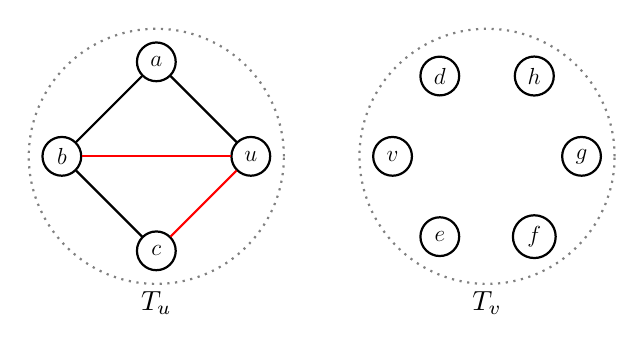
\begin{tikzpicture}
            [scale=0.6, node/.style={scale=0.7, circle,draw,minimum size=2em, thick, font=\large},
            edge/.style={thick, black},
            reserve/.style={red, thick},
            removed/.style={black, thick, dashed}]

            \node[node] (u) at (-1,2) {$u$};
            \node[node] (a) at (-3,4) {$a$};
            \node[node] (b) at (-5,2) {$b$};
            \node[node] (c) at (-3,0) {$c$};
            \node[node] (v) at (2,2) {$v$};
            \node[node] (d) at (3,3.7) {$d$};
            \node[node] (e) at (3,0.3) {$e$};
            \node[node] (f) at (5,0.3) {$f$};
            \node[node] (g) at (6, 2) {$g$};
            \node[node] (h) at (5, 3.7) {$h$};
            
            
            % Dotted circles for T_u and T_v
            \draw[dotted, thick, gray] (-3,2) circle (2.7cm);
            \draw[dotted, thick, gray] (4,2) circle (2.7cm);  
            
            % Labels for the circles
            \node at (-3,-1.1) {$T_u$};
            \node at (4,-1.1) {$T_v$};
            
            \draw[reserve] (b) -- (u) node[midway, below] {};
            \draw[reserve] (c) -- (u) node[midway, below] {};
            \draw[edge] (a) -- (u) node[midway, below] {};
            \draw[edge] (a) -- (b) node[midway, below] {};
            \draw[edge] (b) -- (c) node[midway, below] {};

        \end{tikzpicture}
    \end{minipage}
    \caption{Representação da busca por uma aresta substituta em $R_4$. As arestas reservas de nível $4$ que estão tracejadas foram percorridas e estão prestes a ser removidas de $R_4$, pois foram rebaixadas para o nível $3$, com se pode ver em $R_3$.}
    \vspace{-1cm}
    \label{fig:example-replacement3}
\end{figure}


Supondo que achamos a aresta $ad$ como substituta de nível $4$ antes de $cv$, conectamos $T_u$ e $T_v$ chamando \texttt{adicioneFD($F_4$, a, d)} e $ad$ passa a ser uma aresta da floresta, ou seja, é removida de $R_4$. Como $i = 4$ é o nível máximo do grafo nesse exemplo, não precisamos chamar esta rotina para os níveis $i$ superiores e então terminamos a execução do algoritmo. A Figura~\ref{fig:example-replacement4} ilustra essa etapa do algoritmo.

\begin{figure}[H]
    \centering

    \noindent
    \begin{minipage}[c]{2cm}
        \raggedright
        Nível $4$
    \end{minipage}%
    \begin{minipage}[c]{0.8\textwidth}
        \centering
        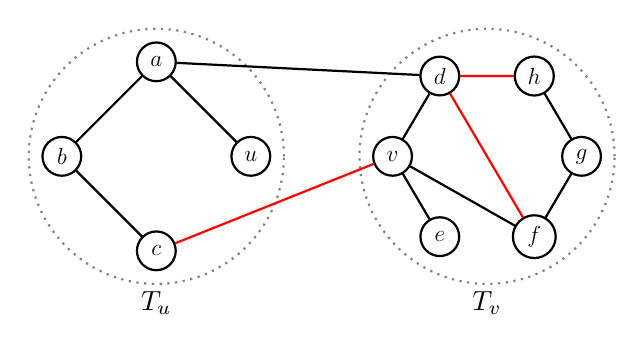
\begin{tikzpicture}
        [scale=0.6, node/.style={scale=0.7, circle,draw,minimum size=2em, thick, font=\large},
        edge/.style={thick, black},
        reserve/.style={red, thick},
        removed/.style={black, thick, dashed}, 
        reserveremoved/.style={red, thick, dashed}]

        \node[node] (u) at (-1,2) {$u$};
        \node[node] (a) at (-3,4) {$a$};
        \node[node] (b) at (-5,2) {$b$};
        \node[node] (c) at (-3,0) {$c$};
        \node[node] (v) at (2,2) {$v$};
        \node[node] (d) at (3,3.7) {$d$};
        \node[node] (e) at (3,0.3) {$e$};
        \node[node] (f) at (5,0.3) {$f$};
        \node[node] (g) at (6, 2) {$g$};
        \node[node] (h) at (5, 3.7) {$h$};
        
         % Dotted circles for T_u and T_v
        \draw[dotted, thick, gray] (-3,2) circle (2.7cm);
        \draw[dotted, thick, gray] (4,2) circle (2.7cm);  
        
        % Labels for the circles
        \node at (-3,-1.1) {$T_u$};
        \node at (4,-1.1) {$T_v$};

        % tree edges (normal black edges)
        \draw[edge] (a) -- (u) node[midway, below] {};
        \draw[edge] (a) -- (b) node[midway, below] {};
        \draw[edge] (b) -- (c) node[midway, below] {};
        \draw[edge] (v) -- (d) node[midway, below] {};
        \draw[edge] (v) -- (f) node[midway, below] {};
        \draw[edge] (v) -- (e) node[midway, below] {};
        \draw[edge] (f) -- (g) node[midway, below] {};
        \draw[edge] (g) -- (h) node[midway, below] {};
        % reserve edges (normal red edges)
        
        \draw[edge] (a) -- (d) node[midway, below] {};
        \draw[reserve] (c) -- (v) node[midway, below] {};
        \draw[reserve] (d) -- (f) node[midway, below] {};
        \draw[reserve] (d) -- (h) node[midway, below] {};

        \end{tikzpicture}
    \end{minipage}
    \vspace{1cm}
        \noindent
    \begin{minipage}[c]{2cm}
        \raggedright
        Nível $3$
    \end{minipage}%
    \begin{minipage}[c]{0.8\textwidth}
        \centering
        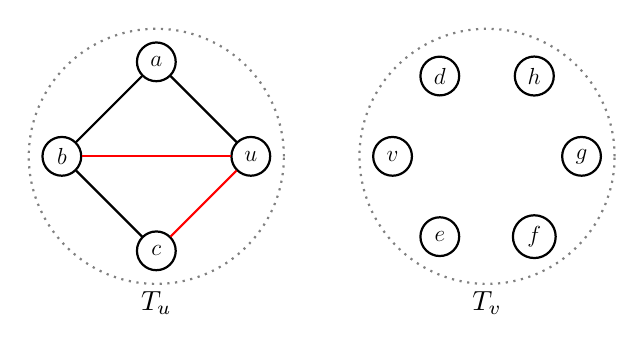
\begin{tikzpicture}
            [scale=0.6, node/.style={scale=0.7, circle,draw,minimum size=2em, thick, font=\large},
            edge/.style={thick, black},
            reserve/.style={red, thick},
            removed/.style={black, thick, dashed}]

            \node[node] (u) at (-1,2) {$u$};
            \node[node] (a) at (-3,4) {$a$};
            \node[node] (b) at (-5,2) {$b$};
            \node[node] (c) at (-3,0) {$c$};
            \node[node] (v) at (2,2) {$v$};
            \node[node] (d) at (3,3.7) {$d$};
            \node[node] (e) at (3,0.3) {$e$};
            \node[node] (f) at (5,0.3) {$f$};
            \node[node] (g) at (6, 2) {$g$};
            \node[node] (h) at (5, 3.7) {$h$};
            
            
            % Dotted circles for T_u and T_v
            \draw[dotted, thick, gray] (-3,2) circle (2.7cm);
            \draw[dotted, thick, gray] (4,2) circle (2.7cm);  
            
            % Labels for the circles
            \node at (-3,-1.1) {$T_u$};
            \node at (4,-1.1) {$T_v$};
            
            \draw[reserve] (b) -- (u) node[midway, below] {};
            \draw[reserve] (c) -- (u) node[midway, below] {};
            \draw[edge] (a) -- (u) node[midway, below] {};
            \draw[edge] (a) -- (b) node[midway, below] {};
            \draw[edge] (b) -- (c) node[midway, below] {};

        \end{tikzpicture}
    \end{minipage}
    \caption{Representação do grafo com a aresta substituta $ad$ escolhida para conectar $T_u$ a $T_v$ em $F_4$, tornando-se uma aresta da floresta.}
    \vspace{-1cm}
    \label{fig:example-replacement4}
\end{figure}

Quando removemos uma aresta da floresta de nível $i$ que quebra uma componente da floresta $F_i$ em duas, note que ao procurar por uma aresta substituta não necessariamente percorreremos todas as arestas reservas em $R_i$. Então nem sempre todas as arestas reservas de $R_i$ são rebaixadas, visto que o algoritmo será finalizado no momento em que encontrarmos uma substituta.

O Programa~\ref{prog:removeGD} apresenta uma primeira versão da rotina \texttt{removaGD}. Note que ele contém uma chamada à rotina \texttt{substituaAresta} que será explicada Seção~\ref{sec:replace-edge}. Alguns ajustes em \texttt{removaGD} serão necessários devido à implementação da rotina \texttt{substituaAresta}. 
Além disso, falta apresentar a estratégia usada para percorrer as arestas da floresta e reservas de forma eficiente. Isso será descrito nas Seções~\ref{sec:node-edge}~e~\ref{sec:node-vertex}.

\begin{programruledcaption}{\texttt{removaGD($G$, $u$, $v$)} \label{prog:removeGD}}
    \noindent\textbf{Entrada}: Recebe dois vértices $u$ e $v$ adjacentes do grafo $G$. \\
    \noindent\textbf{Efeito}: Remove a aresta $uv$ do grafo $G$. 
    \vspace{-0.5\baselineskip}
    \begin{lstlisting}[
        language={[brazilian]pseudocode},
        style=pseudocode,
        style=wider,
        functions={},
        specialidentifiers={},
        escapeinside={(*@}{@*)},
    ]
    i := G.nível[u, v]
    nível[u, v] := \texttt{NIL} (*@\hfill $\triangleright$ marcamos uv como removida@*)
    \textbf{se} uv $\in$ G.$F_{\left\lceil \lg n \right\rceil}$ \textbf{então}  (*@\hfill $\triangleright$ uv é aresta da floresta@*)
        \textbf{para} j := i \textbf{até} $\left\lceil \lg n \right\rceil$ \textbf{faça}
            \texttt{removaFD($G.F_j$, $u$, $v$)}
        \texttt{substituaAresta($G$, $i$, $u$, $v$)}
    \textbf{senão} (*@\hfill $\triangleright$ uv é aresta reserva@*)
        \texttt{removaLA($G.R_i$, $u$, $v$)}
    \end{lstlisting}
    \vspace{-0.5\baselineskip}
\end{programruledcaption}









































\section{Estrutura interna do grafo dinâmico}
\label{sec:dynamic-graph-implementation}

\subsection{Euler tour trees}
\label{sec:euler-tour-trees}

A Seção~2.1 do artigo de Holm, de Lichtenberg e Thorup~\cite{jacob_holm} propõe o uso de Euler tour trees, que é uma técnica utilizada para representar uma árvore. Essa representação é obtida de uma árvore $T$ substituindo-se cada aresta por dois arcos em sentidos opostos e adicionando-se um laço a cada vértice, como pode ser visto na Figura~\ref{fig:euler-tour-trees}. O digrafo resultante é Euleriano, ou seja, é conexo e o grau de entrada de cada vértice é igual ao grau de saída. Como consequência, cada componente uma trilha que começa e termina num mesmo vértice, passando por todos os arcos do digrafo somente uma vez. Tal trilha é chamada de \textbf{ciclo Euleriano}.

\begin{figure}[H]
    \centering
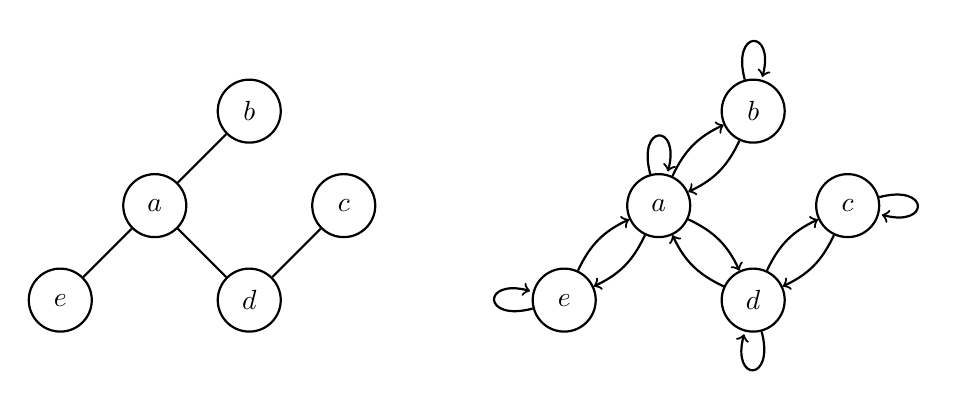
\begin{tikzpicture}[scale=0.8, thick, node distance=2cm,
  vtx/.style={draw, circle, minimum size=8mm, inner sep=0pt}]

% ---------- Left: original graph ----------
\node[vtx] (a) at (0,0) {$a$};
\node[vtx] (b) at (1.5,1.5) {$b$};
\node[vtx] (c) at (3,0) {$c$};
\node[vtx] (d) at (1.5,-1.5) {$d$};
\node[vtx] (e) at (-1.5,-1.5) {$e$};

% Graph edges
\draw (a) -- (b);
\draw (c) -- (d);
\draw (d) -- (a);
\draw (a) -- (e);

% \node[vtx] (a) at (0,0) {$a$};
% \node[vtx] (b) at (1.5,1.5) {$b$};
% \node[vtx] (c) at (3,0) {$c$};
% \node[vtx] (d) at (1.5,-1.5) {$d$};
% \node[vtx] (e) at (-1.5,-1.5) {$e$};

% ---------- Right: Euler-tour representation ----------
\begin{scope}[xshift=8cm]
  \node[vtx] (a1) at (0,0) {$a$};
  \node[vtx] (b1) at (1.5, 1.5) {$b$};
  \node[vtx] (c1) at (3,0) {$c$};
  \node[vtx] (d1) at (1.5,-1.5) {$d$};
  \node[vtx] (e1) at (-1.5,-1.5) {$e$};

  % Bidirectional arcs
  \draw[->] (a1) to[bend left=20] (b1);
  \draw[->] (b1) to[bend left=20] (a1);

  \draw[->] (c1) to[bend left=20] (d1);
  \draw[->] (d1) to[bend left=20] (c1);

  \draw[->] (d1) to[bend left=20] (a1);
  \draw[->] (a1) to[bend left=20] (d1);

  \draw[->] (a1) to[bend left=20] (e1);
  \draw[->] (e1) to[bend left=20] (a1);

  \draw[->] (a1) edge[loop above] ();
  \draw[->] (b1) edge[loop above] ();
  \draw[->] (c1) edge[loop right] ();
  \draw[->] (d1) edge[loop below] ();
  \draw[->] (e1) edge[loop left] ();

\end{scope}

\end{tikzpicture}
    \caption{À esquerda, temos uma árvore $T$ e, à direita, temos o digrafo Euleriano de $T$.}
    \label{fig:euler-tour-trees}
\end{figure}

\raggedbottom

A representação da árvore $T$ é basicamente a sequência de arcos que forma um ciclo Euleriano do digrafo correspondente a $T$. Denotamos cada arco pelo par de vértices que o compõe. Dessa forma, se o arco parte de $u$ para $v$, ele será denotado como $uv$. Para o caso do laço em um vértice $u$, então o arco será escrito como $uu$. Assim, no exemplo da Figura~\ref{fig:euler-tour-trees}, um possível ciclo Euleriano poderia ser o seguinte: 

\setcounter{equation}{0}
    
\begin{equation}
\textit{ee ea aa ab bb ba ad dd dc cc cd da ae}
\label{eq:euler-sequence}
\end{equation}

A sequência dos arcos obtida de $T$ pode mudar dependendo do vértice inicial e da ordem em que os vizinhos de cada vértice são visitados. Uma tal sequência é chamada \textbf{sequência Euleriana} de $T$. 

Henzinger e King \cite{henzinger_king} propuseram armazenar uma sequência Euleriana em uma árvore binária balanceada, usando como chave a posição de cada elemento na sequência. Tomando como base o nosso exemplo da árvore da Figura~\ref{fig:euler-tour-trees} e sua sequência euleriana dada em~\ref{eq:euler-sequence}, podemos ilustrar uma possível árvore binária balanceada para ela na Figura~\ref{fig:euler-tour-balanced-tree}.

\begin{figure}[H]
    \centering
    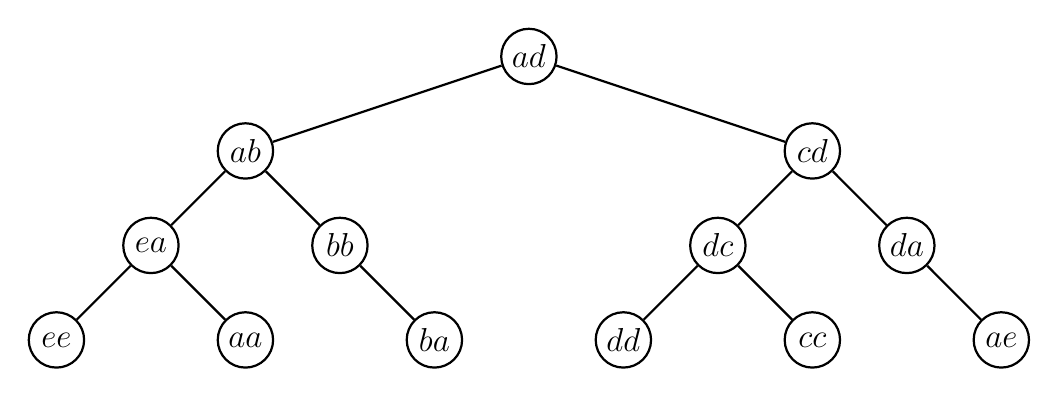
\begin{tikzpicture}
        [scale=0.8, node/.style={circle,draw,minimum size=2em, thick, font=\large},
        edge/.style={thick, black},
        reserve/.style={red, thick},
        removed/.style={black, thick, dashed}, 
        inner sep=0pt]

        \node[node] (ad) at (0, 0) {$ad$};
        \node[node] (ab) at (-4.5, -1.5) {$ab$};
        \node[node] (cd) at (4.5, -1.5) {$cd$};
        \node[node] (dc) at (3, -3) {$dc$};
        \node[node] (dd) at (1.5, -4.5) {$dd$};
        \node[node] (cc) at (4.5, -4.5) {$cc$};
        
        
        
        \node[node] (da) at (6, -3) {$da$};
        \node[node] (ae) at (7.5, -4.5) {$ae$};
        
        
        \node[node] (ea) at (-6, -3) {$ea$};
        \node[node] (ee) at (-7.5, -4.5) {$ee$};
        \node[node] (aa) at (-4.5, -4.5) {$aa$};


        \node[node] (bb) at (-3, -3) {$bb$};
        \node[node] (ba) at (-1.5, -4.5) {$ba$};

        

        % tree edges (normal black edges)
        \draw[edge] (ad) -- (ab) node[midway, below] {};
        \draw[edge] (ad) -- (cd) node[midway, below] {};
        \draw[edge] (cd) -- (dc) node[midway, below] {};
        \draw[edge] (cd) -- (da) node[midway, below] {};
        \draw[edge] (bb) -- (ba) node[midway, below] {};
        \draw[edge] (ea) -- (ee) node[midway, below] {};
        \draw[edge] (ea) -- (aa) node[midway, below] {};
        \draw[edge] (dc) -- (dd) node[midway, below] {};
        \draw[edge] (dc) -- (cc) node[midway, below] {};
        \draw[edge] (da) -- (ae) node[midway, below] {};

        \draw[edge] (ab) -- (ea) node[midway, below] {};
        \draw[edge] (ab) -- (bb) node[midway, below] {};


    \end{tikzpicture}
    \caption{Uma árvore binária balanceada para um ciclo Euleriano da árvore da Figura~\ref{fig:euler-tour-trees}. Note que se percorrermos os nós da árvore acima em \textit{inorder}, obtemos a sequência Euleriana de \ref{eq:euler-sequence}.}
    \label{fig:euler-tour-balanced-tree}
\end{figure}

\raggedbottom

Além disso, Henzinger e King \cite{henzinger_king} propuseram representar uma floresta pela coleção de árvores para sequências eulerianas Eulerianas de cada componente da floresta. Assim, é possível implementar as operações de consulta de conexidade e de alteração na floresta com consumo esperado de tempo $\Oh(\lg n)$ (amortizado em nossa implementação), onde $n$ é o número de nós da floresta. O algoritmo de Holm, de Lichtenberg e Thorup~\cite{jacob_holm} armazena cada floresta $F_i$ com uma estrutura dessas.

\subsection{Nós das florestas}
\label{sec:graph-nodes}

Os nós das árvores de busca binária que representam as sequências Eulerianas das florestas, que são mantidas pelo nosso grafo, serão chamados de \textbf{nós das florestas}. Cada tal nó pode representar um vértice $u$ do grafo, se o elemento armazenado no nó for $uu$, ou pode representar uma aresta $uv$ do grafo, se o elemento armazenado no nó for $uv$ ou $vu$, com $u \neq v$. O primeiro tipo de nó é chamado de \textbf{nó de vértice} e o segundo, de \textbf{nó de aresta}. Em nossa implementação, usaremos um mapa hash \textit{nó} que armazena, para cada par de vértices $(u, v)$, um apontador para o nó do elemento $uv$ na floresta, se tal nó existe (ou \texttt{NIL} caso não exista).

Como representamos uma Euler tour tree por uma árvore binária, cada nó possui apontadores para o filho esquerdo, filho direito e o pai do nó. Em nossa implementação, denotamos tais apontadores por \textit{nó.filhoEsq}, \textit{nó.filhoDir} e \textit{nó.pai}, respectivamente. O motivo de usar um apontador para o pai do nó será discutido depois. A seguir, descreveremos a funcionalidade de cada tipo de nó, bem como outros atributos relevantes que lhe pertencem. 

\subsection{Nó de aresta}
\label{sec:node-edge}

Como já observamos, na floresta $F_i$, há arestas de nível $\leq i$. Para percorrermos as arestas de nível $i$ de uma componente de $F_i$ eficientemente, os nós da floresta $F_i$ tem um atributo extra booleano chamado \textit{éNível}, que indica se tal aresta da floresta $F_i$ é de nível $i$. Além disso, todos os nós da floresta armazenam um contador chamado \textit{arestasDeNível}, com a quantidade de nós de arestas em sua subárvore que têm o \textit{éNível} verdadeiro. Sempre que modificarmos a floresta, vamos acionar uma rotina auxiliar que atualiza este contador e que está descrita no Programa~\ref{prog:updateIsLevelCount-GD}.

\begin{programruledcaption}{\texttt{atualizeArestasDeNível($\emph{nó}$)} \label{prog:updateIsLevelCount-GD}}
    \noindent\textbf{Entrada}: Recebe um nó de aresta.\\
    \noindent\textbf{Efeito}: Atualiza o contador \textit{arestasDeNível} do nó e de seus ascendentes.
    \vspace{-0.5\baselineskip}
    \begin{lstlisting}[
        language={[brazilian]pseudocode},
        style=pseudocode,
        style=wider,
        functions={},
        specialidentifiers={},
        escapeinside={(*@}{@*)},
    ]
    \textbf{enquanto} nó.pai $\neq$ \texttt{NIL} \textbf{faça}
        c := 0
        \textbf{se} nó.filhoEsq $\neq$ \texttt{NIL} \textbf{então}
            c := c + \textit{nó.filhoEsq.arestasDeNível}
        \textbf{se} nó.filhoDir $\neq$ \texttt{NIL} \textbf{então}
            c := c + \textit{nó.filhoDir.arestasDeNível}
        \textbf{se} nó.éNível \textbf{então}
            c := c + 1
        nó.arestasDeNível := c
        nó := nó.pai
\end{lstlisting}
\vspace{-0.5\baselineskip}
\end{programruledcaption}

Como se pode ver no Programa~\ref{prog:updateIsLevelCount-GD}, precisamos atualizar o contador \textit{arestasDeNível} do nó e o de seus ascendentes. Por isso, precisamos do campo \textit{pai} para percorrer até a raiz da árvore. Como a nossa implementação usa árvores \textit{splay}, então acionamos a operação \texttt{splay} no nó em questão e atualizamos este contador. como se pode ver no Programa~\ref{prog:updateIsLevelCount-GD-splay}.

\begin{programruledcaption}{\texttt{atualizeArestasDeNível($\emph{nó}$)} \label{prog:updateIsLevelCount-GD-splay}}
    \noindent\textbf{Entrada}: Recebe um nó de aresta.\\
    \noindent\textbf{Efeito}: Atualiza o contador \textit{arestasDeNível} do nó e de seus ascendentes.
    \vspace{-0.5\baselineskip}
    \begin{lstlisting}[
        language={[brazilian]pseudocode},
        style=pseudocode,
        style=wider,
        functions={},
        specialidentifiers={},
        escapeinside={(*@}{@*)},
    ]
    \texttt{splay($\emph{nó}$)}
    c := 0
    \textbf{se} nó.filhoEsq $\neq$ \texttt{NIL} \textbf{então}
        c := c + \textit{nó.filhoEsq.arestasDeNível}
    \textbf{se} nó.filhoDir $\neq$ \texttt{NIL} \textbf{então}
        c := c + \textit{nó.filhoDir.arestasDeNível}
    \textbf{se} nó.éNível \textbf{então}
        c := c + 1
    nó.arestasDeNível := c
\end{lstlisting}
\vspace{-0.5\baselineskip}
\end{programruledcaption}

O Programa~\ref{prog:updateIsLevelCount-GD} consome tempo $\Oh(\lg n)$ e Programa~\ref{prog:updateIsLevelCount-GD-splay} consome tempo amortizado $\Oh(\lg n)$. Veja que ambos os programas não alteram a árvore e, portanto, todas as três invariantes são preservadas. 

Usando o mesmo exemplo da Figura~\ref{fig:euler-tour-balanced-tree} na Seção~\ref{sec:euler-tour-trees}, podemos ilustrar como estaria o atributo \textit{arestasDeNível} de cada nó na árvore. Na nossa implementação, os vértices são identificados por inteiros de $1$ a $n$ e, para uma aresta $uv$, usamos o atributo \textit{éNível} apenas para o nó de $uv$ com $u < v$.

\begin{figure}[H]
    \centering
    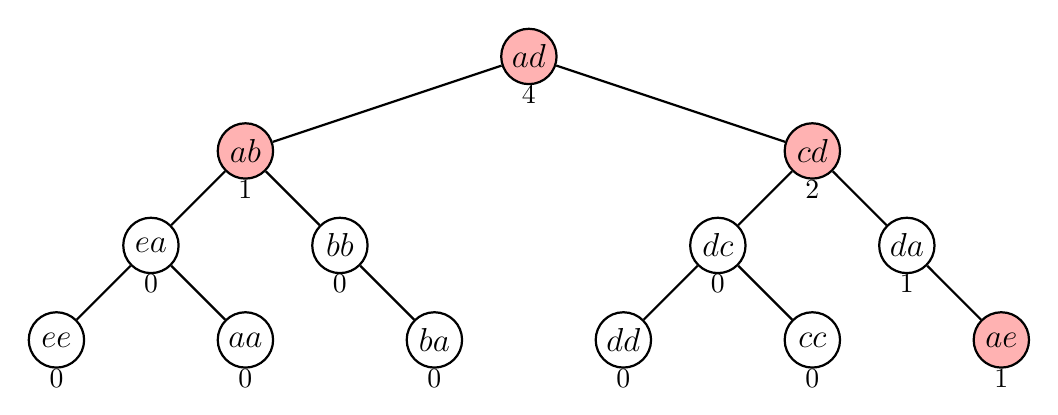
\begin{tikzpicture}
        [scale=0.8, node/.style={circle,draw,minimum size=2em, thick, font=\large},
        edge/.style={thick, black},
        reserve/.style={red, thick},
        removed/.style={black, thick, dashed}, 
        inner sep=0pt]

        \node[node, fill=red!30, label=below:{4}] (ad) at (0, 0) {$ad$};
        \node[node, fill=red!30, label=below:{1}] (ab) at (-4.5, -1.5) {$ab$};
        \node[node, fill=red!30, label=below:{2}] (cd) at (4.5, -1.5) {$cd$};
        \node[node, label=below:{0}] (dc) at (3, -3) {$dc$};
        \node[node, label=below:{0}] (dd) at (1.5, -4.5) {$dd$};
        \node[node, label=below:{0}] (cc) at (4.5, -4.5) {$cc$};
        
        
        \node[node, label=below:{1}] (da) at (6, -3) {$da$};
        \node[node, fill=red!30, label=below:{1}] (ae) at (7.5, -4.5) {$ae$};
        
        
        \node[node, label=below:{0}] (ea) at (-6, -3) {$ea$};
        \node[node, label=below:{0}] (ee) at (-7.5, -4.5) {$ee$};
        \node[node, label=below:{0}] (aa) at (-4.5, -4.5) {$aa$};


        \node[node, label=below:{0}] (bb) at (-3, -3) {$bb$};
        \node[node, label=below:{0}] (ba) at (-1.5, -4.5) {$ba$};

        

        % tree edges (normal black edges)
        \draw[edge] (ad) -- (ab) node[midway, below] {};
        \draw[edge] (ad) -- (cd) node[midway, below] {};
        \draw[edge] (cd) -- (dc) node[midway, below] {};
        \draw[edge] (cd) -- (da) node[midway, below] {};
        \draw[edge] (bb) -- (ba) node[midway, below] {};
        \draw[edge] (ea) -- (ee) node[midway, below] {};
        \draw[edge] (ea) -- (aa) node[midway, below] {};
        \draw[edge] (dc) -- (dd) node[midway, below] {};
        \draw[edge] (dc) -- (cc) node[midway, below] {};
        \draw[edge] (da) -- (ae) node[midway, below] {};

        \draw[edge] (ab) -- (ea) node[midway, below] {};
        \draw[edge] (ab) -- (bb) node[midway, below] {};


    \end{tikzpicture}
    \caption{Árvore de uma das componentes da floresta $F_i$, onde nós pintados em vermelho indicam arestas de nível $i$, e logo possuem o atributo éNível verdadeiro. Embaixo de cada nó temos o valor do contador arestasDeNível.}
    \label{fig:euler-tour-balanced-tree-is-level-propagation}
\end{figure}

Na Figura~\ref{fig:euler-tour-balanced-tree-is-level-propagation}, note que os nós $\emph{ab}$ e $\emph{ba}$ representam a mesma aresta. Assim, para evitar a duplicação do atributo \textit{éNível}, optamos por colocar este atributo como verdadeiro somente nos nós de aresta cujos vértices estão em ordem lexicográfica. Então, no nosso exemplo, nós do tipo $\emph{ba}$, $\emph{da}$, $\emph{dc}$ e $\emph{ea}$ vão ter este atributo falso. 

Lembre-se que, durante a remoção de uma aresta $uv$ de nível $i$ da floresta $F_i$, quebramos uma componente de $F_i$ em duas, $T_u$ e $T_v$. Sendo $T_u$ a menor das duas, precisamos realizar o rebaixamento das arestas de nível $i$ de $T_u$ para $i-1$. Para fazer isso de forma eficiente, introduzimos um método auxiliar chamado \texttt{procureArestaDeNível}. Esse método utiliza o atributo \textit{arestasDeNível} para encontrar um a um, numa árvore da floresta $F_i$, os nós de arestas de nível $i$.

\begin{programruledcaption}{\texttt{procureArestaDeNível(\textit{nó})} \label{prog:findEdgesIsLevel-GD}}
    \noindent\textbf{Entrada}: Recebe um nó de uma floresta com o contador \textit{arestasDeNível} $> 0$.
    \\
    \noindent\textbf{Saída}: Devolve um nó de aresta da subárvore do nó com \textit{éNível} verdadeiro.
    \vspace{-0.5\baselineskip}
    \begin{lstlisting}[
        language={[brazilian]pseudocode},
        style=pseudocode,
        style=wider,
        functions={},
        specialidentifiers={},
        escapeinside={(*@}{@*)},
    ]
    \textbf{se} nó.éNível \textbf{então}
        devolva nó
    \textbf{se} nó.filhoEsq $\neq$ \texttt{NIL} \textbf{e} nó.filhoEsq.arestasDeNível > 0 \textbf{então}
        devolva \texttt{procureArestaDeNível($\emph{nó.filhoEsq}$)}
    \textbf{senão}
        devolva \texttt{procureArestaDeNível($\emph{nó.filhoDir}$)}
\end{lstlisting}
\vspace{-0.5\baselineskip}
\end{programruledcaption}

Veja que o Programa~\ref{prog:findEdgesIsLevel-GD} não altera o grafo, e, portanto, as invariantes são preservadas. Como a Euler tour tree é balanceada, então o consumo de tempo de cada percurso é $\Oh(\lg n)$ (amortizado em nossa implementação). Assim, se temos $k$ arestas de nível $i$ da árvore a serem rebaixadas, então a busca por essas $k$ arestas custará tempo $\Oh(k \lg n)$.

\subsection{Nó de vértice}
\label{sec:node-vertex}

Para percorrermos as arestas reservas de nível $i$ incidentes a vértices da árvore $T_u$ em busca de uma aresta substituta, cada nó do tipo vértice $u$ (ou $uu$) possui um booleano chamado \textit{incideArestaReservaDeNível} que indica se $u$ é uma das pontas de alguma aresta reserva de nível $i$. Dessa forma, se $uv$ é aresta reserva de nível $2$, então os nós de vértice $u$ e $v$ em $F_2$ terão o atributo \textit{incideArestaReservaDeNível} como verdadeiro. 

Todos os nós da floresta também guardarão um contador \textit{arestasReservasDeNível}, a fim de calcular a quantidade de nós em sua subárvore que tenham o booleano \textit{incideArestaReservaDeNível} verdadeiro. Esse contador é constantemente atualizado durante a adição e remoção de arestas, e para isso precisamos de uma rotina auxiliar \texttt{atualizeArestasReservasDeNível} descrito no Programa~\ref{prog:updateReserveEdgesCount-GD}. 

\begin{programruledcaption}{\texttt{atualizeArestasReservasDeNível($\emph{nó}$)} \label{prog:updateReserveEdgesCount-GD}}
    \noindent\textbf{Entrada}: Recebe um nó de vértice.
    \\
    \noindent\textbf{Efeito}: Atualiza o contador \textit{arestasReservasDeNível} do nó de vértice $u$.
    \vspace{-0.5\baselineskip}
    \begin{lstlisting}[
        language={[brazilian]pseudocode},
        style=pseudocode,
        style=wider,
        functions={},
        specialidentifiers={},
        escapeinside={(*@}{@*)},
    ]
    \textbf{enquanto} nó.pai $\neq$ \texttt{NIL} \textbf{faça}
        c := 0
        \textbf{se} nó.filhoEsq $\neq$ \texttt{NIL} \textbf{então}
            c := c + nó.filhoEsq.arestasReservasDeNível
        \textbf{se} nó.filhoDir $\neq$ \texttt{NIL} \textbf{então}
            c := c + nó.filhoDir.arestasReservasDeNível
        \textbf{se} nó.incideArestaReservaDeNível  \textbf{então}
            c := c + 1
        nó.arestasReservasDeNível := c
        nó := nó.pai
    \end{lstlisting}
    \vspace{-0.5\baselineskip}
\end{programruledcaption}

\raggedbottom

Similarmente ao Programa~\ref{prog:updateIsLevelCount-GD-splay}, o Programa~\ref{prog:updateReserveEdgesCount-GD} na nossa implementação também acionamos \texttt{splay}, mas neste caso atualizamos o atributo \textit{arestasReservasDeNível}, como se pode ver no Programa~\ref{prog:updateReserveEdgesCount-splay-GD}. 

\begin{programruledcaption}{\texttt{atualizeArestasReservasDeNível($\emph{nó}$)} \label{prog:updateReserveEdgesCount-splay-GD}}
    \noindent\textbf{Entrada}: Recebe um nó de vértice.
    \\
    \noindent\textbf{Efeito}: Atualiza o contador \textit{arestasReservasDeNível} do nó de vértice $u$.
    \vspace{-0.5\baselineskip}
    \begin{lstlisting}[
        language={[brazilian]pseudocode},
        style=pseudocode,
        style=wider,
        functions={},
        specialidentifiers={},
        escapeinside={(*@}{@*)},
    ]
    \texttt{splay($\emph{nó}$)}
    c := 0
    \textbf{se} nó.filhoEsq $\neq$ \texttt{NIL} \textbf{então}
        c := c + nó.filhoEsq.arestasReservasDeNível
    \textbf{se} nó.filhoDir $\neq$ \texttt{NIL} \textbf{então}
        c := c + nó.filhoDir.arestasReservasDeNível
    \textbf{se} nó.incideArestaReservaDeNível  \textbf{então}
        c := c + 1
    nó.arestasReservasDeNível := c
    \end{lstlisting}
    \vspace{-0.5\baselineskip}
\end{programruledcaption}

O Programa~\ref{prog:updateReserveEdgesCount-GD} consome tempo $\Oh(\lg n)$ e o Programa~\ref{prog:updateReserveEdgesCount-splay-GD} consome tempo amortizado $\Oh(\lg n)$. Como não há alteração do grafo, então as três invariantes são preservadas.

Usando o mesmo exemplo da Figura~\ref{fig:euler-tour-balanced-tree} na Seção~\ref{sec:euler-tour-trees}, podemos ilustrar como estaria o atributo \textit{arestasReservasDeNível} de cada nó na árvore.

\begin{figure}[H]
    \centering
    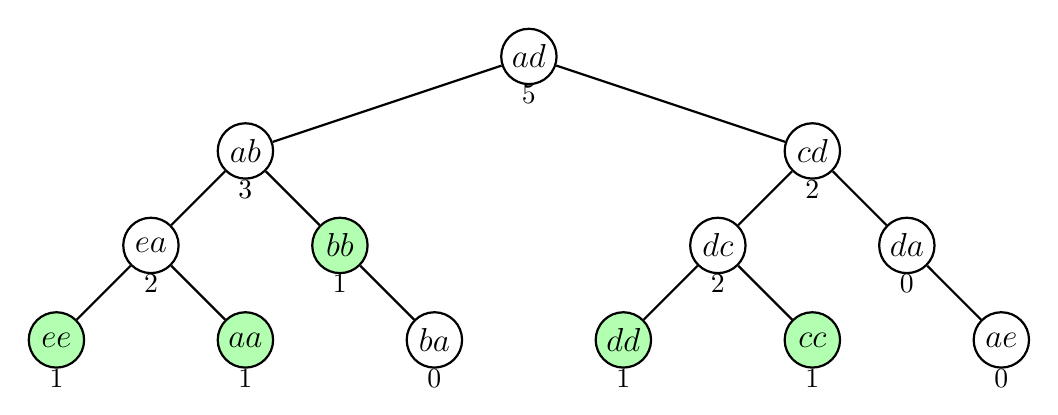
\begin{tikzpicture}
        [scale=0.8, node/.style={circle,draw,minimum size=2em, thick, font=\large},
        edge/.style={thick, black},
        reserve/.style={red, thick},
        removed/.style={black, thick, dashed}, 
        inner sep=0pt]

        \node[node, label=below:{5}] (ad) at (0, 0) {$ad$};
        \node[node, label=below:{3}] (ab) at (-4.5, -1.5) {$ab$};
        \node[node, label=below:{2}] (cd) at (4.5, -1.5) {$cd$};
        \node[node, label=below:{2}] (dc) at (3, -3) {$dc$};
        \node[node, fill=green!30, label=below:{1}] (dd) at (1.5, -4.5) {$dd$};
        \node[node, fill=green!30, label=below:{1}] (cc) at (4.5, -4.5) {$cc$};
        
        
        \node[node, label=below:{0}] (da) at (6, -3) {$da$};
        \node[node, label=below:{0}] (ae) at (7.5, -4.5) {$ae$};
        
        
        \node[node, label=below:{2}] (ea) at (-6, -3) {$ea$};
        \node[node, fill=green!30, label=below:{1}] (ee) at (-7.5, -4.5) {$ee$};
        \node[node, fill=green!30, label=below:{1}] (aa) at (-4.5, -4.5) {$aa$};


        \node[node, fill=green!30, label=below:{1}] (bb) at (-3, -3) {$bb$};
        \node[node, label=below:{0}] (ba) at (-1.5, -4.5) {$ba$};

        

        % tree edges (normal black edges)
        \draw[edge] (ad) -- (ab) node[midway, below] {};
        \draw[edge] (ad) -- (cd) node[midway, below] {};
        \draw[edge] (cd) -- (dc) node[midway, below] {};
        \draw[edge] (cd) -- (da) node[midway, below] {};
        \draw[edge] (bb) -- (ba) node[midway, below] {};
        \draw[edge] (ea) -- (ee) node[midway, below] {};
        \draw[edge] (ea) -- (aa) node[midway, below] {};
        \draw[edge] (dc) -- (dd) node[midway, below] {};
        \draw[edge] (dc) -- (cc) node[midway, below] {};
        \draw[edge] (da) -- (ae) node[midway, below] {};

        \draw[edge] (ab) -- (ea) node[midway, below] {};
        \draw[edge] (ab) -- (bb) node[midway, below] {};


    \end{tikzpicture}
    \caption{Árvore de uma das componentes da floresta $F_i$, onde nós pintados em verde indicam vértices com o atributo incideArestaReservaDeNível verdadeiro. No nosso exemplo, todos os vértices são ponta de alguma aresta reserva de nível $i$. Embaixo de cada nó temos o contador arestasReservasDeNível.}
    \label{fig:euler-tour-balanced-tree-reserve-edges-propagation}
\end{figure}

\raggedbottom

Após vermos esses campos extras que adicionamos nos nós da floresta, perceba que o atributo \textit{éNível} existe em nó de vértice, porém vai ser sempre falso. Da mesma forma, o atributo \textit{incideArestaReservaDeNível} existe em nó de aresta, e vai ser sempre falso também. 

Lembre-se que, após rebaixarmos as arestas de nível $i$ de $T_u$ na etapa da remoção de uma aresta da floresta $F_i$, precisamos procurar por uma aresta substituta. Para isso, precisamos buscar por uma aresta reserva de nível $i$, de modo que uma de suas pontas esteja em $T_u$ e outra em $T_v$, para que consigamos reconectar as duas componentes separadas. 

Para resolver este problema de maneira eficiente, introduzimos um método auxiliar chamado \texttt{procureNóIncideArestaReservaDeNível}, que irá procurar um vértice que incide em uma das arestas reservas de nível $i$.
Essa rotina devolve um vértice $u$ que incide a uma das arestas reservas de nível $i$. Assim, podemos percorrer em $R_i$ cada vizinho $v$ de $u$ para verificar se $uv$ liga $T_u$ a $T_v$. 

\begin{programruledcaption}{\texttt{procureNóIncideArestaReservaDeNível(\textit{nó})} \label{prog:findReserveEdge-GD}}
    \noindent\textbf{Entrada}: Recebe um nó da floresta com o contador \textit{arestasReservasDeNível} $> 0$.
    \\
    \noindent\textbf{Saída}: Devolve um nó de vértice da subárvore do nó com \textit{incideArestaReservaDeNível} verdadeiro.
    \vspace{-0.5\baselineskip}
    \begin{lstlisting}[
        language={[brazilian]pseudocode},
        style=pseudocode,
        style=wider,
        functions={},
        specialidentifiers={},
        escapeinside={(*@}{@*)},
    ]
    \textbf{se} nó.incideArestaReservaDeNível \textbf{então}
        devolva nó
    \textbf{se} nó.filhoEsq $\neq$ \texttt{NIL} \textbf{e} nó.filhoEsq.arestasReservasDeNível > 0 \textbf{então}
        devolva \texttt{procureNóIncideArestaReservaDeNível($\emph{nó.filhoEsq}$)}
    \textbf{senão}
        devolva \texttt{procureNóIncideArestaReservaDeNível($\emph{nó.filhoDir}$)}
\end{lstlisting}
\vspace{-0.5\baselineskip}
\end{programruledcaption}

Veja que o Programa~\ref{prog:findReserveEdge-GD} não altera o grafo, e, portanto, as invariantes são preservadas. Como a Euler tour tree é balanceada, então o consumo de tempo do Programa~\ref{prog:findReserveEdge-GD} é $\Oh(\lg n)$ (amortizado em nossa implementação).

O campo \textit{incideArestaReservaDeNível} de um nó de vértice $u$ pode mudar de valor quando houver inserções e remoções de arestas reservas que possuem como uma da suas pontas o vértice $u$. Portanto, mostraremos dois métodos que modificam este campo e atualizam o contador \textit{arestasReservasDeNível}.

O Programa~\ref{prog:decrementReserveEdgesCount-GD} atualiza o campo \textit{incideArestaReservaDeNível} de um nó de vértice $u$ para falso quando ele não tem mais elementos em sua lista de adjacências, isto é, quando não há mais nenhuma aresta reserva incidente nele. A assinatura \texttt{R[u]} retorna o conjunto de vizinhos da lista de adjacências de $u$.

\begin{programruledcaption}{\texttt{decrementeArestasReservasDeNível($F$, $R$, $u$)} \label{prog:decrementReserveEdgesCount-GD}}
    \noindent\textbf{Entrada}: Recebe um vértice $u$ da floresta $F$ e uma lista de adjacências $R$.\\
    \noindent\textbf{Efeito}: Atualiza o campo \textit{incideArestaReservaDeNível} para falso se necessário.
    \vspace{-0.5\baselineskip}
    \begin{lstlisting}[
        language={[brazilian]pseudocode},
        style=pseudocode,
        style=wider,
        functions={},
        specialidentifiers={},
        escapeinside={(*@}{@*)},
        ]
        vérticeU := F.nó[u, u]
        \textbf{se} R[u] = $\emptyset$ \textbf{então} 
            vérticeU.incideArestaReservaDeNível := falso
            \texttt{atualizeIncideArestaReservaDeNível($\emph{vérticeU}$)}
    \end{lstlisting}
    \vspace{-0.5\baselineskip}
\end{programruledcaption}

Já o Programa~\ref{prog:incrementReserveEdgesCount-GD} atualiza o atributo \textit{incideArestaReservaDeNível} de um nó de vértice $u$ para verdadeiro quando adicionamos um vértice $v$ na lista de adjacências de $u$ e $v$ é o primeiro elemento de sua lista de adjacências, pois isso indica que $u$ passa a ser incidente à aresta reserva $uv$.

\begin{programruledcaption}{\texttt{incrementeArestasReservasDeNível($F$, $R$, $u$)} \label{prog:incrementReserveEdgesCount-GD}}
    \noindent\textbf{Entrada}: Recebe um vértice $u$ da floresta $F$ e uma lista de adjacências $R$.\\
    \noindent\textbf{Efeito}: Atualiza o campo \textit{incideArestaReservaDeNível} para verdadeiro se necessário.
    \vspace{-0.5\baselineskip}
    \begin{lstlisting}[
        language={[brazilian]pseudocode},
        style=pseudocode,
        style=wider,
        functions={},
        specialidentifiers={},
        escapeinside={(*@}{@*)},
    ]
    vérticeU := F.nó[u, u]
    \textbf{se} |R[u]| = $1$ \textbf{então} 
        vérticeU.incideArestaReservaDeNível := verdadeiro
        \texttt{atualizeIncideArestaReservaDeNível($\emph{vérticeU}$)}
    \end{lstlisting}
    \vspace{-0.5\baselineskip}
\end{programruledcaption}


As rotinas \texttt{decrementeArestasReservasDeNível} e \texttt{incrementeArestasReservasDeNível} consomem tempo $\Oh(\lg n)$, amortizado em nossa implementação. Como tais rotinas auxiliares não fazem nenhuma modificação nas florestas do grafo, então todas as invariantes são mantidas. 

\subsection{Segunda versão da rotina de adição de arestas}
\label{sec:code-edge-addition-second-version}

Apresentada a Seção~\ref{sec:node-vertex}, precisamos ajustar o método de adição de arestas (\texttt{adicioneGD}), apresentado no Programa~\ref{prog:addGD-version2}. Atualizamos os atributos desses nós que descrevemos para fazermos a remoção eficiente de arestas, cuja rotina será descrita também com ajustes na Seção~\ref{sec:code-edge-removal-second-version}. Note que o método \texttt{adicioneGD} continua tendo o mesmo consumo de tempo após esses ajustes. 

\begin{programruledcaption}{\texttt{adicioneGD($G$, $u$, $v$)} \label{prog:addGD-version2}}
    \noindent\textbf{Entrada}: Recebe dois vértices $u$ e $v$ do grafo $G$, com $u < v$. \\
    \textbf{Efeito}: Adiciona a aresta $uv$ no grafo $G$.
    \vspace{-0.5\baselineskip}
    \begin{lstlisting}[
        language={[brazilian]pseudocode},
        style=pseudocode,
        style=wider,
        functions={},
        specialidentifiers={},
        escapeinside={(*@}{@*)},
    ]
    G.nível[u, v] := $\left\lceil \lg n \right\rceil$
    \textbf{se} \texttt{conectadosFD($G.F_{\left\lceil \lg n \right\rceil}$, $u$, $v$)} \textbf{então}
        \texttt{adicioneLA($G.R_{\left\lceil \lg n \right\rceil}$, $u$, $v$)}
        \texttt{incrementeArestasReservasDeNível($G.F_{\left\lceil \lg n \right\rceil}$, $G.R_{\left\lceil \lg n \right\rceil}$, $u$)}
        \texttt{incrementeArestasReservasDeNível($G.F_{\left\lceil \lg n \right\rceil}$, $G.R_{\left\lceil \lg n \right\rceil}$, $v$)}
    \textbf{senão}
        \texttt{adicioneFD($G.F_{\left\lceil \lg n \right\rceil}$, $u$, $v$)}
        arestaUV := G.F.nó[u, v]
        arestaUV.éNível := verdadeiro
    \end{lstlisting}
    \vspace{-0.5\baselineskip}
\end{programruledcaption}

Podemos notar algumas diferenças entre as duas versões de \texttt{adicioneGD}. As linhas $4$ e $5$ são necessárias para que os campos \textit {incideArestaReservaDeNível} e \textit{arestasReservasDeNível} dos vértices $u$ e $v$ estejam corretos, pois ao adicionar uma aresta reserva $uv$, precisamos verificar se $u$ e $v$ não eram incidentes a alguma aresta reserva (que seria $uv$), mas passaram a ser. Já as linhas $8$ e $9$ definem o atributo \textit{éNível} da aresta $uv$ como verdadeiro, quando ela é aresta da floresta. 

\subsection{Segunda versão da rotina de remoção de arestas}
\label{sec:code-edge-removal-second-version}

Apresentada a Seção~\ref{sec:node-vertex}, precisamos também ajustar o método de remoção de arestas (\texttt{removaGD}), apresentado no Programa~\ref{prog:removeGD-version2}. 

\begin{programruledcaption}{\texttt{removaGD($G$, $u$, $v$)} \label{prog:removeGD-version2}}
    \noindent\textbf{Entrada}: Recebe dois vértices $u$ e $v$ do grafo $G$. \\
    \noindent\textbf{Efeito}: Remove a aresta $uv$ do grafo $G$. 
    \vspace{-0.5\baselineskip}
    \begin{lstlisting}[
        language={[brazilian]pseudocode},
        style=pseudocode,
        style=wider,
        functions={},
        specialidentifiers={},
        escapeinside={(*@}{@*)},
    ]
    i := G.nível[u, v]
    nível[u, v] := \texttt{NIL} (*@\hfill $\triangleright$ marcamos uv como removida@*)
    \textbf{se} uv $\in$ G.$F_{\left\lceil \lg n \right\rceil}$ \textbf{então}  (*@\hfill $\triangleright$ uv é aresta da floresta@*)
        \textbf{para} j := i \textbf{até} $\left\lceil \lg n \right\rceil$ \textbf{faça}
            \texttt{removaFD($G.F_j$, $u$, $v$)}
        \texttt{substituaAresta($G$, $i$, $u$, $v$)}
    \textbf{senão} (*@\hfill $\triangleright$ uv é aresta reserva@*)
        \texttt{removaLA($G.R_i$, $u$, $v$)}
        \texttt{decrementeArestasReservasDeNível($G.F_i$, $G.R_i$, $u$)}
        \texttt{decrementeArestasReservasDeNível($G.F_i$, $G.R_i$, $v$)}
    \end{lstlisting}
    \vspace{-0.5\baselineskip}
\end{programruledcaption}

A diferença entre as duas versões de \texttt{removaGD} é que a segunda tem as linhas $9$ e $10$ a mais. Tais linhas são necessárias para que o campo \textit{incideArestaReservaDeNível} e o contador \textit{arestasReservasDeNível} estejam corretas, visto que, ao remover uma aresta reserva, precisamos verificar se os vértices incidentes à ela ainda são incidentes a alguma outra. 

Agora falta descrever a rotina \texttt{substituaAresta}, que veremos a seguir que consome tempo amortizado $\Oh(\lg^2 n)$. Consequentemente, \texttt{removaGD} também consumirá tempo amortizado $\Oh(\lg^2 n)$.

\subsection{Rotina de substituição de aresta}
\label{sec:replace-edge}

A rotina de substituição da aresta da floresta está descrita no Programa~\ref{prog:replaceGD}.

\begin{programruledcaption}{\texttt{substituaAresta($G$, $i$, $u$, $v$)} \label{prog:replaceGD}}
    \noindent\textbf{Entrada}: Recebe dois vértices $u$ e $v$ do grafo $G$, e o nível $i$ da aresta $uv$. \\
    \noindent\textbf{Efeito}: Adiciona uma aresta substituta no grafo, se ela existir.
    \vspace{-0.5\baselineskip}
    \begin{lstlisting}[
        language={[brazilian]pseudocode},
        style=pseudocode,
        style=wider,
        functions={},
        specialidentifiers={},
        escapeinside={(*@}{@*)},
    ]
    \textbf{para} j := i \textbf{até} $\left\lceil \lg n \right\rceil$ \textbf{faça}
        $T_u$ := \texttt{árvore($G.F_j.\textit{nó}[u, u]$)}
        $T_v$ := \texttt{árvore($G.F_j.\textit{nó}[v, v]$)}    
        \textbf{se} |$T_u$| > |$T_v$| \textbf{então}
            u $\leftrightarrow$ v
            $T_u \leftrightarrow T_v$
        \textbf{enquanto} raiz($T_u$).arestasDeNível > 0 \textbf{faça} 
            arestaXY := \texttt{procureArestaDeNível(raiz($T_u$))}
            \texttt{rebaixeNívelDaAresta($G$, $\emph{arestaXY}$, j)}
        \textbf{enquanto} raiz($T_u$).arestasReservasDeNível > 0     \textbf{faça}
            vérticeX := \texttt{procureNóIncideArestaReservaDeNível(raiz($T_u$))}
            x := vérticeX[1]
            \textbf{para} $y \in G.R[x]$ \textbf{faça}
                \texttt{removaLA($G.R_j$, $x$, $y$)} 
                \textbf{se} \texttt{conectadosGD($G$, $x$, $y$)} \textbf{então} 
                    G.nível[x, y] := j - 1
                    \texttt{adicioneLA($G.R_{j-1}$, $x$, $y$)}
                    \texttt{incrementeArestasReservasDeNível($G.F_{j-1}$, $G.R_{j-1}$, $x$)}
                    \texttt{incrementeArestasReservasDeNível($G.F_{j-1}$, $G.R_{j-1}$, $y$)}
                \textbf{senão}
                    \textbf{para} k := j \textbf{até} $\left\lceil \lg n \right\rceil$ \textbf{faça}
                        \texttt{adicioneFD($G.F_k$, $x$, $y$)}
                    \textbf{devolva}
    \end{lstlisting}
    \vspace{-0.5\baselineskip}
\end{programruledcaption}

Para explicar o Programa~\ref{prog:replaceGD}, descreveremos a função de cada trecho do código. Lembre-se que, ao removermos uma aresta $uv$ da floresta de nível $i$, precisamos procurar uma substituta partindo de $R_i$, e se não encontrarmos, passamos a buscar em $R_{i + 1}, \ldots, R_L$. A linha $1$ faz exatamente essa iteração sobre os níveis $i$ até $L$. Para evitarmos a confusão de usar $i$ ou $j$ (como está escrito no Programa~\ref{prog:replaceGD}) , vamos usar $j$ para explicar cada trecho do código já que é ela que tá iterando sobre o intervalo $[i, \ldots, L]$. Então vamos assumir que estamos removendo a $uv$ de nível $j$, para $j = i, \ldots , L$

Nas linhas $2$ e $3$, obtemos as árvores $T_u$ e $T_v$, que foram derivadas da floresta $F_j$, já que uma componente desta foi quebrada em duas após a remoção de $uv$. O método auxiliar \texttt{árvore($\textit{nó}$)} apenas retorna a árvore que contém nó, e consome tempo amortizado $\Oh(\lg n)$ em nossa implementação. As linhas $4$ a $6$ garantem que $|T_u| \leq |T_v|$. 

Das linhas $7$ a $9$, realizamos o processo de rebaixar todas arestas de $T_u$ de nível $j$. Na linha $7$, temos um laço \textit{while} que irá terminar quando rebaixarmos todas as arestas de nível $j$, isto é, quando o contador \textit{arestasDeNível} do nó raiz de $T_u$ zerar. Para obter a raiz de $T_u$, usamos um outro mapa hash chamado \texttt{raiz}, que mapeia cada árvore ao seu respectivo nó raiz. Então \texttt{raiz(T)} retorna o nó raiz da árvore $T$, e tal mapeamento consome tempo esperado constante.

Na linha $8$, utilizamos o método auxiliar \texttt{procureArestaDeNível}, que irá retornar um nó de aresta de nível $j$, ou seja, que possui o \textit{éNível} verdadeiro. Para cada nó de aresta retornado, rebaixamos-o chamando o método \texttt{rebaixeNívelDaAresta}, descrito no Programa~\ref{prog:decrease-edge-level}.


\begin{programruledcaption}{\texttt{rebaixeNívelDaAresta($G$, $\textit{nó}$, $j$)} \label{prog:decrease-edge-level}}
    \noindent\textbf{Entrada}: Recebe o grafo $G$, um nó de aresta e o nível $j$.\\
    \textbf{Efeito}: Rebaixa o nível do nó de aresta.
    \vspace{-0.5\baselineskip}
    \begin{lstlisting}[
        language={[brazilian]pseudocode},
        style=pseudocode,
        style=wider,
        functions={},
        specialidentifiers={},
        escapeinside={(*@}{@*)},
    ]
    x := nó[1]
    y := nó[2]
    G.nível[x, y] := j - 1
    \texttt{puxeParaRaiz($\emph{nó}$)}
    nó.éNível := falso
    \texttt{atualizeArestasDeNível($G.F_j$, $x$, $y$)}
    \texttt{adicioneFD($G.F_{j-1}$, $x$, $y$)}

    \end{lstlisting}
    \vspace{-0.5\baselineskip}
\end{programruledcaption}

No Programa~\ref{prog:decrease-edge-level}, atualizamos o nível do nó de aresta $xy$ de $j$ para $j-1$. As assinaturas $\emph{nó[1]}$ e $\emph{nó[2]}$ representam as pontas do nó (nesse caso de $xy$), que no nosso exemplo atribuímos às variáveis $x$ e $y$. Ademais, precisamos atualizar o campo \textit{éNível} para falso pois $xy$ não é mais de nível $j$ em $F_j$. Assim, atualizamos o contador \textit{arestasDeNível} acionando a rotina \texttt{atualizeArestasDeNível}, e por fim adicionamos $xy$ em $F_{j-1}$, já que tal aresta foi rebaixada para o nível $j-1$. Veja que \texttt{rebaixeNívelDaAresta} consome tempo amortizado $O(\lg n)$. Se temos $k$ arestas de $T_u$ para rebaixar, as linhas $7$ a $9$ logo consomem tempo $\Oh(k \lg n)$.  

Já nas linhas $10$ a $23$ procuramos por uma aresta substituta de nível $j$. Similarmente à linha $7$, a linha $10$ é um laço \textit{while} que irá terminar quando não existir mais arestas reservas de nível $j$ (ou seja, o contador \textit{arestasReservasDeNível} do nó raiz de $T_u$ é zerado) ou quando achamos uma aresta substituta.  

Na linha $11$, acionamos \texttt{procureNóIncideArestaReservaDeNível}, que irá retornar um nó de vertice $xx$ que incide uma das arestas reservas de nível $i$. Como tanto $\emph{nó[1]}$ quanto $\emph{nó[2]}$ retornam $x$ para um nó de vértice $xx$, escolhemos o primeiro para podermos percorrer todos os vizinhos $y$ de lista de adjacências de $x$ na linha $13$, pois queremos testar se $xy$ é uma potencial aresta substituta.

A linha $14$ remove a aresta reserva $xy$ de $R_j$, independentemente se tal aresta é substituta ou não. Se $xy$ não é substituta, então precisamos rebaixá-la para $R_{j-1}$, como visto na Seção~\ref{sec:dynamic-graph-edge-removal}. Se ela é substituta, então ela vai acabar se tornando uma aresta da floresta que conecta $T_u$ a $T_v$.

As linhas $15$ a $19$ englobam o caso em que os vértices $x$ e $y$ estão em $T_u$, isto é, quando \texttt{conectadosGD(G, x, y)} retorna verdadeiro. Isso quer dizer que $xy$ não é uma aresta substituta, e por isso precisamos rebaixá-la de $R_j$ para $R_{j-1}$, além de atualizar \texttt{incideArestaReservaDeNível} e \texttt{arestasReservasDeNível} de $x$ e de $y$ em $F_{j-1}$. 

Veja que~\texttt{conectadosGD(G, x, y)} só devolverá falso quando $x$ está em $T_u$ e $y$ está em $T_v$, pois assim os dois vértices estariam em componentes separadas. Este caso, abordado nas linhas $20$ a $23$ do Programa~\ref{prog:replaceGD}, mostra que encontramos $xy$ como uma aresta substituta, e finalizamos o algoritmo conectando $x$ de $T_u$ a $y$ de $T_v$ de todas as florestas $F_k$, para $k = j, \ldots, L$, por conta da invariante~\ref{invariant2}.



